\documentclass[a4paper,11pt]{memoir}

% *************** Document style definitions ***************
% *************** Document style definitions ***************

% ******************************************************************
% This file defines the document design.
% Usually it is not necessary to edit this file, but you can change
% the design if you want.
% ******************************************************************

% *************** Load packages ***************
\usepackage{graphicx}
\usepackage{subcaption}
\usepackage{subfig}
%\usepackage{subcaption}
%\usepackage[fleqn]{amsmath}
\usepackage{amssymb}
\usepackage{amsmath}
\usepackage{amsthm}
\usepackage{siunitx} % A comprehensive (SI) units package
\sisetup{% alterado para usar vírgula e não ponto ...
     output-decimal-marker = {,},   
     inter-unit-product = \ensuremath{{}\cdot{}}
        }
\usepackage{eurosym}
\usepackage{booktabs}
\usepackage{fancyvrb}
\usepackage{float}
\usepackage{stmaryrd} %St Mary Road symbols for theoretical computer science
\usepackage{url}
\usepackage{longtable}
\usepackage{multirow}
\usepackage[figuresright]{rotating}
\usepackage[utf8]{inputenc}
\usepackage{aeguill} % to use in french \guillemotleft "«"  and \guillemotright "»" characters
\usepackage{lscape}
\usepackage{tabularx}
\usepackage{hyperref}
\usepackage{makeidx}
\usepackage{citeref} %Add reference-page-list to bibliography-items
\usepackage[portuguese]{babel}  
\selectlanguage{portuguese}

%para fazer as anotações
\usepackage[colorinlistoftodos]{todonotes}


% to load the figures from a folder
\graphicspath{{figuras/}}

% to enable code environment
\floatstyle{ruled}
\newfloat{myprogram}{htbp}{prg}[chapter]
\floatname{myprogram}{Code Snippets} \floatstyle{plain}

%enable 4 sections levels
\setcounter{secnumdepth}{5}

% *************** Enable index generation ***************
\makeindex

% *************** Add reference to page number at which bibliography entry is cited ***************
\usepackage{citeref}
\renewcommand{\bibitempages}[1]{\newblock {\scriptsize [\mbox{cited on p.\ }#1]}}

% *************** Some colour definitions ***************
\usepackage{color}

\definecolor{greenyellow}   {cmyk}{0.15, 0   , 0.69, 0   }
\definecolor{yellow}        {cmyk}{0   , 0   , 1   , 0   }
\definecolor{goldenrod}     {cmyk}{0   , 0.10, 0.84, 0   }
\definecolor{dandelion}     {cmyk}{0   , 0.29, 0.84, 0   }
\definecolor{apricot}       {cmyk}{0   , 0.32, 0.52, 0   }
\definecolor{peach}         {cmyk}{0   , 0.50, 0.70, 0   }
\definecolor{melon}         {cmyk}{0   , 0.46, 0.50, 0   }
\definecolor{yelloworange}  {cmyk}{0   , 0.42, 1   , 0   }
\definecolor{orange}        {cmyk}{0   , 0.61, 0.87, 0   }
\definecolor{burntorange}   {cmyk}{0   , 0.51, 1   , 0   }
\definecolor{bittersweet}   {cmyk}{0   , 0.75, 1   , 0.24}
\definecolor{redorange}     {cmyk}{0   , 0.77, 0.87, 0   }
\definecolor{mahogany}      {cmyk}{0   , 0.85, 0.87, 0.35}
\definecolor{maroon}        {cmyk}{0   , 0.87, 0.68, 0.32}
\definecolor{brickred}      {cmyk}{0   , 0.89, 0.94, 0.28}
\definecolor{red}           {cmyk}{0   , 1   , 1   , 0   }
\definecolor{orangered}     {cmyk}{0   , 1   , 0.50, 0   }
\definecolor{rubinered}     {cmyk}{0   , 1   , 0.13, 0   }
\definecolor{wildstrawberry}{cmyk}{0   , 0.96, 0.39, 0   }
\definecolor{salmon}        {cmyk}{0   , 0.53, 0.38, 0   }
\definecolor{carnationpink} {cmyk}{0   , 0.63, 0   , 0   }
\definecolor{magenta}       {cmyk}{0   , 1   , 0   , 0   }
\definecolor{violetred}     {cmyk}{0   , 0.81, 0   , 0   }
\definecolor{rhodamine}     {cmyk}{0   , 0.82, 0   , 0   }
\definecolor{mulberry}      {cmyk}{0.34, 0.90, 0   , 0.02}
\definecolor{redviolet}     {cmyk}{0.07, 0.90, 0   , 0.34}
\definecolor{fuchsia}       {cmyk}{0.47, 0.91, 0   , 0.08}
\definecolor{lavender}      {cmyk}{0   , 0.48, 0   , 0   }
\definecolor{thistle}       {cmyk}{0.12, 0.59, 0   , 0   }
\definecolor{orchid}        {cmyk}{0.32, 0.64, 0   , 0   }
\definecolor{darkorchid}    {cmyk}{0.40, 0.80, 0.20, 0   }
\definecolor{purple}        {cmyk}{0.45, 0.86, 0   , 0   }
\definecolor{plum}          {cmyk}{0.50, 1   , 0   , 0   }
\definecolor{violet}        {cmyk}{0.79, 0.88, 0   , 0   }
\definecolor{royalpurple}   {cmyk}{0.75, 0.90, 0   , 0   }
\definecolor{blueviolet}    {cmyk}{0.86, 0.91, 0   , 0.04}
\definecolor{periwinkle}    {cmyk}{0.57, 0.55, 0   , 0   }
\definecolor{cadetblue}     {cmyk}{0.62, 0.57, 0.23, 0   }
\definecolor{cornflowerblue}{cmyk}{0.65, 0.13, 0   , 0   }
\definecolor{midnightblue}  {cmyk}{0.98, 0.13, 0   , 0.43}
\definecolor{navyblue}      {cmyk}{0.94, 0.54, 0   , 0   }
\definecolor{royalblue}     {cmyk}{1   , 0.50, 0   , 0   }
\definecolor{blue}          {cmyk}{1   , 1   , 0   , 0   }
\definecolor{cerulean}      {cmyk}{0.94, 0.11, 0   , 0   }
\definecolor{cyan}          {cmyk}{1   , 0   , 0   , 0   }
\definecolor{processblue}   {cmyk}{0.96, 0   , 0   , 0   }
\definecolor{skyblue}       {cmyk}{0.62, 0   , 0.12, 0   }
\definecolor{turquoise}     {cmyk}{0.85, 0   , 0.20, 0   }
\definecolor{tealblue}      {cmyk}{0.86, 0   , 0.34, 0.02}
\definecolor{aquamarine}    {cmyk}{0.82, 0   , 0.30, 0   }
\definecolor{bluegreen}     {cmyk}{0.85, 0   , 0.33, 0   }
\definecolor{emerald}       {cmyk}{1   , 0   , 0.50, 0   }
\definecolor{junglegreen}   {cmyk}{0.99, 0   , 0.52, 0   }
\definecolor{seagreen}      {cmyk}{0.69, 0   , 0.50, 0   }
\definecolor{green}         {cmyk}{1   , 0   , 1   , 0   }
\definecolor{forestgreen}   {cmyk}{0.91, 0   , 0.88, 0.12}
\definecolor{pinegreen}     {cmyk}{0.92, 0   , 0.59, 0.25}
\definecolor{limegreen}     {cmyk}{0.50, 0   , 1   , 0   }
\definecolor{yellowgreen}   {cmyk}{0.44, 0   , 0.74, 0   }
\definecolor{springgreen}   {cmyk}{0.26, 0   , 0.76, 0   }
\definecolor{olivegreen}    {cmyk}{0.64, 0   , 0.95, 0.40}
\definecolor{rawsienna}     {cmyk}{0   , 0.72, 1   , 0.45}
\definecolor{sepia}         {cmyk}{0   , 0.83, 1   , 0.70}
\definecolor{brown}         {cmyk}{0   , 0.81, 1   , 0.60}
\definecolor{tan}           {cmyk}{0.14, 0.42, 0.56, 0   }
\definecolor{gray}          {cmyk}{0   , 0   , 0   , 0.50}
\definecolor{black}         {cmyk}{0   , 0   , 0   , 1   }
\definecolor{white}         {cmyk}{0   , 0   , 0   , 0   }


% *************** Page layout ***************

\settrimmedsize{297mm}{210mm}{*} 
\setlength{\trimtop}{0pt} 
\setlength{\trimedge}{\stockwidth} 
\addtolength{\trimedge}{-\paperwidth} 
\settypeblocksize{*}{420pt}{1.618}
\setulmargins{30mm}{*}{1.618}
\setlrmargins{*}{25mm}{1.618}
%\setmarginnotes{25mm}{25mm}{\onelineskip}
\setheadfoot{\onelineskip}{3\onelineskip}
\setheaderspaces{*}{1.5\onelineskip}{*}
%\def\baselinestretch{1.1}
\checkandfixthelayout 

%%
% *************** Chapter and section style ***************
\makechapterstyle{mychapterstyle}{%
    \renewcommand{\chapnamefont}{\LARGE\sffamily\bfseries}%
    \renewcommand{\chapnumfont}{\LARGE\sffamily\bfseries}%
    \renewcommand{\chaptitlefont}{\Huge\sffamily\bfseries}%
    \renewcommand{\printchaptertitle}[1]{%
        \chaptitlefont\hrule height 0.5pt \vspace{1em}%
        {##1}\vspace{1em}\hrule height 0.5pt%
        }%
    \renewcommand{\printchapternum}{%
    \chapnumfont\thechapter%
    }%
}

\chapterstyle{mychapterstyle}

\setsecheadstyle{\Large\sffamily\bfseries}
\setsubsecheadstyle{\large\sffamily\bfseries}
\setsubsubsecheadstyle{\normalfont\sffamily\bfseries}
\setparaheadstyle{\normalfont\sffamily}

\makeevenhead{headings}{\thepage}{}{\small\slshape\leftmark}
\makeoddhead{headings}{\small\slshape\rightmark}{}{\thepage}


% *************** Table of contents style ***************
\settocdepth{subsubsection} \setsecnumdepth{subsubsection}
\maxsecnumdepth{subsubsection} \settocdepth{subsubsection}
\maxtocdepth{subsubsection}

% ********** Commands for epigraphs **********
\setlength{\epigraphwidth}{0.57\textwidth}
\setlength{\epigraphrule}{0pt}
\setlength{\beforeepigraphskip}{1\baselineskip}
\setlength{\afterepigraphskip}{2\baselineskip}
\setlength{\parskip}{1ex plus 0.5ex minus 0.2ex}

\newcommand{\epitext}{\sffamily\itshape}
\newcommand{\epiauthor}{\sffamily\scshape ---~}
\newcommand{\epititle}{\sffamily\itshape}
\newcommand{\epidate}{\sffamily\scshape}
\newcommand{\episkip}{\medskip}

\newcommand{\myepigraph}[4]{%
    \epigraph{\epitext #1\episkip}{\epiauthor #2\\\epititle #3 \epidate(#4)}\noindent}

% *************** Other ***************
\renewcommand{\thefootnote}{\arabic{footnote}}

\newenvironment{mylisting}
  {\begin{list}{}{\setlength{\leftmargin}{1em}}\item\scriptsize\bfseries}
  {\end{list}}

% ************** Figures **************

\renewcommand{\topfraction}{0.85}
\renewcommand{\textfraction}{0.1}
\renewcommand{\floatpagefraction}{0.75}




% ************** Parâmetros para definição de capa e outros **************
\newcommand{\cursoaux}{teste}
\newcommand{\tituloaux}{}
\newcommand{\organizacaoaux}{}
\newcommand{\alunoaux}{}
\newcommand{\datadefesaaux}{}
\newcommand{\orientadoraux}{}
\newcommand{\supervisoraux}{}


\newcommand{\curso}[1]{\renewcommand{\cursoaux}{#1}}
\newcommand{\titulo}[1]{\renewcommand{\tituloaux}{#1}}
\newcommand{\organizacao}[1]{\renewcommand{\organizacaoaux}{#1}}
\newcommand{\aluno}[1]{\renewcommand{\alunoaux}{#1}}
\newcommand{\datadefesa}[1]{\renewcommand{\datadefesaaux}{#1}}
\newcommand{\orientador}[1]{\renewcommand{\orientadoraux}{#1}}
\newcommand{\supervisor}[1]{\renewcommand{\supervisoraux}{#1}}

\newif\ifestagio





% *************** Headers and Footers ***************
\makeevenhead{headings}{\thepage\hrule}{}{\footnotesize\tituloaux\hrule}
\makeoddhead{headings}{\footnotesize\tituloaux\hrule}{}{\thepage\hrule}
\makeevenfoot{headings}{\hrule\footnotesize\slshape\rightmark}{}{\hrule\footnotesize\alunoaux}
\makeoddfoot{headings}{\hrule\footnotesize\alunoaux}{}{\hrule\footnotesize\slshape\rightmark}

% *************** End of document style definition ***************

\begin{document}

% *************** Hifenização ***************
\hyphenation{
    ca-pa-ci-da-de
    }

% *************** Título do projeto, aluno, orientador, etc. ************

\curso{Licenciatura em Engenharia de Sistemas}
\titulo{DESENVOLVIMENTO DE UM SISTEMA DE INFORMAÇÃO DE FÁBRICA}
\organizacao{Natural Life, Lda.}
\aluno{Jorge Gabriel Azevedo (1160929)}
\datadefesa{19 de julho de 2019}
\orientador{Prof. Manuel Carlos Felgueiras}
% no caso de projeto interno não há supervisor
% desativar flag de estagio
\estagiotrue 
%\estagiofalse
\supervisor{Engº Telmo Azevedo}  % é ignorado quando flag desativada

% *************** Front matter ********************
\frontmatter
% *************** Capa do relatório ***************
% *************** Title page ****************
% *** utiliza variáveis cujos valores são ***
% ***  definidas no documento principal   *** 

\pagestyle{empty} \sffamily \noindent

\begin{center}
    
\reversemarginpar

    \begin{figure}[H]
        \centering
\includegraphics[width=12.0cm]{figuras/ISEP_logo.jpg}
    \end{figure}

    % dados do trabalho
    
    \textbf{\huge \cursoaux}
    \vskip15mm

    \begin{table}[htb]
    \renewcommand\arraystretch{8}
    \centering
        \begin{tabular}{>{\centering\arraybackslash}m{13.5cm} }
            \textbf{\huge\tituloaux}\par\\
         \end{tabular}
    \end{table}    

    \vskip5mm
    \textbf{\Large \organizacaoaux}

    \vspace*{\stretch{3}}
    \vskip10mm
    \textbf{\LARGE \alunoaux}

    \vspace*{\stretch{3}}
    \vspace*{4mm} 
    \textbf{\Large \datadefesaaux}

    \vskip10mm
   
    \Large{Orientador ISEP: \textbf{\orientadoraux}}

    \vskip5mm
    \ifestagio
    \Large{Supervisor Externo: \textbf{\supervisoraux}}
    \fi
\end{center}

\cleardoublepage


% ***************
\pagenumbering{roman} \pagestyle{headings}
% *************** Agradecimentos *******************
%\addcontentsline{toc}{chapter}{Agradecimentos}
% ********** Agradecimentos **********
\chapter*{Agradecimentos}

Agradecimentos que sejam devidos. Esta secção é opcional!

% ********** End of Acknowledgements **********
\cleardoublepage
% *************** Portuguese Abstract **************
\addcontentsline{toc}{chapter}{Resumo}
% ********** Resumo **********
\chapter*{Resumo}

O uso de velas de cera é uma prática muito comum em Portugal. Estas são usadas para as mais variadíssimas atividades, mas o tratamento dos resíduos provenientes da queima da vela não são devidamente tratados. Não existindo solução para estes resíduos, eles acabam em aterros poluindo ainda mais o nosso planeta. Neste sentido existem empresa como a Natural Life, lda que procedem à recolha destes residuos e posterior reciclagem. Sendo esta uma atividade bastante especifica, o uso de um software ERP genérico pode trazer muita ineficiência ao processo.
Neste documento é descrito o processo de desenvolvimento de um sistema de gestão dos recursos adequado ao processo da empresa Natural Life.

\textbf{Palavras-Chave}: Velas, Cera, NaturalLife, Reciclagem, ERP, Projeto/Estágio, Engenharia de Sistemas, ISEP.

% ********** End of Resumo **********
\todo{Fazer o resumo}
\cleardoublepage
% *************** English Abstract *****************
%\addcontentsline{toc}{chapter}{Abstract}
%% ********** Abstract **********
\chapter*{Abstract}

The abstract should summarize the report’s contents, in what concerns the problem identification and/or the formulated hypotheses. The solution, its validation and assessment should also be briefly focused. In all, it should be less than 2 pages in length.

\textbf{Keywords:} We would like to encourage you to list your keywords, key phrases and most relevant acronyms in this section.

% ********** End of Abstract **********
%\cleardoublepage
% *************** Table of contents ****************
\renewcommand*\contentsname{Índice}
\tableofcontents
\cleardoublepage
% *************** Table of figures *****************
\renewcommand{\listfigurename}{Índice de figuras}
\listoffigures 
\cleardoublepage
% *************** Table of tables ******************
\renewcommand{\listtablename}{Índice de tabelas}
\listoftables 
\cleardoublepage
% *************** Table of symbols *****************
% *************** List of symbols and abbreviations ***************

% ******************************************************************************
% You can make list of symbols and abbreviations here.
% You only need to make a label when a symbol is introduced in the document and
% here you can reference this label to obtain page number.
% ******************************************************************************

\chapter[Acrónimos]{Acrónimos}

\begin{center}
\small
\begin{longtable}{lp{3.0in}c}
\toprule \multicolumn{1}{c}{Acrónimo} 
                & \multicolumn{1}{c}{Descrição}
                                & \multicolumn{1}{c}{Página}\\ \midrule\addlinespace[2pt] \endhead

\bottomrule\endfoot

ERP		& Enterprise Resource Planning			& \pageref{sym:ERP}\\
MVC		& Model View Controller					& \pageref{sym:MVC}\\
PROES	& Unidade Curricular Projeto / Estágio	& \pageref{sym:PROES}\\
SI		& Sistema de Informação					& \pageref{sym:SI}\\
TI		& Tecnologias de Informação				& \pageref{sym:TI}\\


\end{longtable}

\end{center}

% *************** End of list of symbols and abbreviations ***************
\cleardoublepage
% *************** Main matter **********************
\mainmatter
% ************ Capítulo 1 ************
%\renewcommand{\chaptername}{Capítulo}
\chapter{Introdução}
\label{cap:1}

\section{Enquadramento}
Em Portugal o uso de vela de cera é uma pratica bastante recorrente. Estas são usadas para iluminação, como elementos decorativos e para o culto ao mortos. Todos os anos milhares de velas são utilizadas em território nacional, nomeadamente círios. Os círios são particularmente frequentes em cemitérios. Constituídos por um envolucro em plástico e com uma tampa em metal são vistos como elemento obrigatório na homenagem a um ente querido falecido. Pela quantidade de velas que são queimadas diariamente os resíduos destas amontoam-se e a solução que é vista para este problema é o colocar o que resta do círio no caixote do lixo indiferenciado. Esta situação acarreta vários problemas ambientais que a médio prazo podem ter consequências mais gravosas, como por exemplo, infestação de vespas e abelhas uma vez que estes animais usam a cera das velas para construir as suas estruturas de abrigo.
A reciclagem de resíduos de velas ainda não é neste momento uma atividade com grande expressão no mercado Português. Existem apenas algumas empresas atualmente a fazer a reciclagem deste tipo de resíduos e as suas principais fontes de materia-prima são os cemitérios e locais de culto religioso, onde o uso de velas é uma pratica muito comum. Entre as entidades que operam neste setor podemos mencionar o Santuário de Fátima\cite{Destak2010}, o Centro Ambiental do Carvalho de Calvos\cite{SecundinoCunha2016} e a Natural Life\cite{NaturalLife}.

\section{Apresentação da empresa}
A Natural Life, Lda. é uma empresa fundada em 2013. Está sediada na rua de Terramonte nº 781, Armazém C20, na Maia. Tendo como atividade a recolha e reciclagem de resíduos de velas, a Natural Life surge como uma empresa ecológica, inteiramente ligada a área ambiental, mais concretamente à reciclagem\cite{NaturalLife}. A empresa cuida de todo o processo, desde a recolha da materia-prima nos cemitérios com as quais tem parceria, a separação do corpo de plastico, da tampa de metal e da cera até à fundição da cera. Em alguns casos a recolha do material é substituída por material recolhido por terceiros, mantendo-se o resto do processo. A fábrica está dividida em duas áreas especificas: a zona de armazém, cargas e descargas e a zona de processamento dos círios. Os registos da fábrica são feitos numa base de dados muito simples, com vários tipos de limitações que inibem a empresa de poder expandir.

\section{Objetivos}
Implementar um sistema de informação (SI\label{sym:SI}) para efetuar o registo do ponto dos colaboradores, recolhas, produção, acabamento e saída do produto. Esta solução teria de possuir duas áreas distintas, a primeira destinada ao uso na fábrica e a segunda destinada ao uso pela administração. Pretende-se ainda que esta seja uma solução bem integrada no processo da empresa e que traga o leve tempo possível de adaptação ao novo sistema por parte dos funcionários.

\section{Calendarização}
Para descrever a calendarização da Unidade Curricular (UC\label{sym:UC}) PROjeto/EStágio (PROES\label{sym:PROES}) da Licenciatura em Engenharia de Sistemas (LES\label{sym:LES}).

\begin{figure}[htbp] 
	\begin{center}
		% Requires \usepackage{graphicx}
		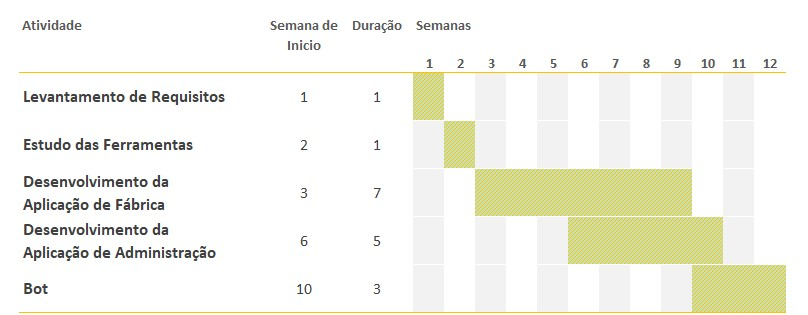
\includegraphics[width=\textwidth,keepaspectratio]{figuras/DiagramaGant.jpg}
		\caption{Planemento - diagrama de Gantt}
		\label{fig:gantt chart} 
	\end{center}
\end{figure}

\section{Organização do relatório}
No Capítulo 1 é feito o enquadramento do projeto dando uma visão alto nível do projeto. No capítulo 2, é apresentado o estado da arte. É neste capitulo que são descritas as diferentes opções para a realização do projeto e onde são descritas as escolhas feitas e o seu motivo. No capítulo 3 é apresentada a lista de requisitos e do projeto, bem como o processo para a sua obtenção. O capítulo 4, destina-se à projeção do sistema descrevendo o modo como os elementos do sistema se interligam entre si, para no capítulo 5 ser descrito o processo de implementação e a sua validação. No último capítulo, o 6º, são apresentadas as conclusões do projeto. É ainda neste capitulo que é feita a analise critica do estudante face ao trabalho desenvolvido.

\cleardoublepage
% ************ Chapter 2 ************
\chapter{Contexto} 
\label{cap:2}

\section{Estado da arte}
Existem varias ferramentas para fazer a gestão dos recursos de uma empresa e cada uma com as suas características. Para analisar as opções disponíveis, selecionou-se algumas aplicações ERP de forma a poder comparar os seus recursos com as necessidades da empresa.

\subsection{SAP ERP}
SAP ERP  é um sistema integrado de gestão empresarial (ERP) transacional, produto principal da empresa alemã SAP AG líder no segmento de software corporativos.\cite{Wikipediab}. É uma aplicação composta por módulos, nos quais cada modulo é responsável por uma parte da atividade da empresa.


\subsection{Primavera Executive}
O PRIMAVERA Executive é um software ERP desenvolvido pela empresa PRIMAVERA Business Software Solutions com foco nas pequenas e médias empresas \cite{PRIMAVERABSS}. A PRIMAVERA Business Software Solutions é uma empresa que se dedica ao desenvolvimento e comercialização de soluções de gestão e plataformas para integração de processos empresariais \cite{Wikipediaa}. Esta tecnológica portuguesa que se afirmou no mercado nacional de soluções informáticas de gestão por ser pioneira no desenvolvimento de aplicações para Windows. \cite{Wikipediaa}.
Esta solução inclui ainda integração com os softwares de faturação PRIMAVERA.

\subsection{Microsoft Dynamics}
Microsoft Dynamics é um pacote software da Microsoft destinado a gestão corporativa ERP, para ajudar na tomada de decisões gerenciais e melhorar os resultados administrativos e financeiros das empresas.\cite{Wikipediac}
Dentro deste pacote de software existem as seguintes aplicações:
\begin{itemize}
	\item Dynamics 365 for Sales
	\item Dynamics 365 for Retail
	\item Dynamics 365 for Finance and Operations
	\item Dynamics 365 for Talent
\end{itemize}
Este pacote está disponível em várias edições nas quais varia as funcionalidades disponíveis de modo a se ajustar melhor às necessidades da empresa.

\section{Tabela comparativa}
A informação coletada sobre as diferentes opções foi colocada na tabela \ref{tab:opcoes_mercado}

\begin{longtable}{|m{0.30\textwidth}|m{0.10\textwidth}|m{0.10\textwidth}|m{0.10\textwidth}|m{0.20\textwidth}|}
	\hline
	Característica & SAP & \specialcell{Primavera\\Executive} & \specialcell{Microsoft\\Dynamics} & Solução Própria\\ \hline
	Funções de gestão 
	de recursos da empresa		& \ding{51} & \ding{51} & \ding{51} & \ding{51}\\ \hline
	Acesso remoto externo		& \ding{51} & \ding{51} & \ding{51} & \ding{53}\\ \hline
	Suporte técnico de terceiros& \ding{51} & \ding{51} & \ding{51} & \ding{53}\\ \hline
	Controlo do desenvolvimento & \ding{53} & \ding{53} & \ding{53} & \ding{51}\\ \hline
	Atualizações do sistema		& \ding{51} & \ding{51} & \ding{51} & tem de as
																	desenvolver\\ \hline
	Adaptação total do sistema
	às necessidades da empresa	& \ding{53} & \ding{53} & \ding{53} & \ding{51}\\ \hline
	Implementação apenas dos recursos necessário
								& \ding{53} & \ding{53} & \ding{53} & \ding{51}\\ \hline
	\caption{Tabela resumo das opções}
	\label{tab:opcoes_mercado}
\end{longtable}

\section{Opção escolhida}
No final desta analise, o caminho definido para o projeto foi a criação de uma nova plataforma, sendo que essa era a intenção da empresa desde o incio. Por esse motivo foi feita uma nova analise de opções à cerca do desenvolvimento da plataforma. Este documento foi entregue à administração para que o analisa-se o decidisse o modo como a aplicação deveria ser desenvolvida. O documento entregue esta presente no \hyperref[anexo:A]{Anexo A}. Desse documento é possível extrair a tabela comparativa com as diferentes opções para o desenvolvimento da plataforma. Essa tabela é apresentada na tabela \ref{tab:opcoes_dev}.


\begin{longtable}{|p{0.20\textwidth}|p{0.15\textwidth}|p{0.25\textwidth}|p{0.25\textwidth}|}
	\hline
	& Opção                                                 & Vantagens                                                           & Desvantagens                                                                                        \\ \hline
	\multirow{6}{*}{Tipo de Aplicação}                                      & \multirow{3}{*}{Desktop}                              &                                                                     & Necessidade de configurar cada computador que receber a aplicação                                   \\
	&                                                       &                                                                     & Parar o computador para atualizar a aplicação                                                       \\
	&                                                       &                                                                     & Necessidade de um servidor de base de dados                                                         \\ \cline{2-4}
	& \multirow{3}{*}{Web}                                  & Acesso direto em qualquer computador                                & Necessidade de um servidor web e de base de dados                                                   \\
	&                                                       & Maior familiaridade com a plataforma por parte de programador       &                                                                                                     \\
	&                                                       & Menos pontos de falha                                               &                                                                                                     \\ \hline
	
	\multirow{5}{*}{Sistema Operativo}                                      & \multirow{3}{*}{Windows 10}                           & Familiaridade com o sistema                                         & Necessidade de comprar uma licença do Windows Server                                                \\
	&                                                       & Todas as máquinas já executam esta plataforma                       & Necessidade de aprender ASP.NET ou usar o XAMPP                                                     \\
	&                                                       &                                                                     & Se não for usado só software Microsoft não há garantias de segurança/ compatibilidade com o Windows \\ \cline{2-4} 
	& \multirow{2}{*}{Ubuntu 18.04}                         & Plataforma líder de mercado                                         & Curva de aprendizagem para manutenção básica                                                        \\
	&                                                       & Milhares de pacotes no repositório que são revisados pela Canonical &                                                                                                     \\ \hline
	
	\multirow{10}{*}{\specialcell{Sistema de Gestão\\de\\Base de Dados}}    & \multirow{3}{*}{\specialcell{Microsoft SQL\\Server}}  & Familiaridade com o software                                        & Versão Express limitada.                                                                            \\
	&                                                       & Versão Express gratuita                                             & Versões Enterprise e Standard pagas                                                                 \\
	&                                                       &                                                                     & Versão Developer não utilizável em produção                                                         \\ \cline{2-4}
	& \multirow{7}{*}{MariaDB}                              & Gratuito (versão Open Source)                                       & Não possui um ficheiro único para a base de dados.                                                  \\
	&                                                       & Totalmente compatível com MySQL da Oracle                           & Tem de ser instalado manualmente no Windows ou usado com recurso ao XAMPP                           \\
	&                                                       & Padrão no Ubuntu e no XAMPP                                         &                                                                                                     \\
	&                                                       & Escalável                                                           &                                                                                                     \\
	&                                                       & Fiável                                                              &                                                                                                     \\
	&                                                       & Recursos semelhante ao MS SQL Server                                &                                                                                                     \\
	&                                                       & Suporte nativo no Ubuntu                                            &                                                                                                     \\ \hline
	
	\multirow{5}{*}{Tipo de Máquina}                                        & \multirow{2}{*}{Real}                                 & Não dependência da operação de outras máquinas                      & Hardware dedicado                                                                                   \\
	&                                                       &                                                                     &                                                                                                     \\ \cline{2-4}
	& \multirow{3}{*}{Virtual}                              & Não necessita de hardware dedicado.                                 & Exige que o utilizador que esta a executar a VM nunca termine a sessão.                             \\
	&                                                       & Várias instâncias da máquina ao mesmo tempo.                        & Se a máquina real tiver de ser reiniciada, a VM tem de ser interrompida                             \\
	&                                                       & Backup muito fácil.                                                 & Partilha dos recursos da máquina hospedeira com a maquina virtual.                                  \\
	\hline
	\caption{Tabela resumo das opções}
	\label{tab:opcoes_dev}
\end{longtable}



\section{Analise das opções disponíveis}
O documento entregue incide sobre os aspetos base para a criação do sistema de informação: tipologia de aplicação, servidor, sistema de gestão de base de dados, linguagens de programação.

O primeiro a ser definido seria o tipologia de aplicação. Decidir sobre uma aplicação web ou uma plicação desktop poderia condicionar o trabalho futuro. Aqui a sugestão passou pelo desenvolvimento de uma aplicação web, pois esta seria agnóstica de equipamento o que dava uma grande flexibilidade no futuro. Além deste fator, já se sabia que teria de existir uma máquina servidor pois teria de haver uma base de dados centralizada, logo não havia nenhum gasto extra com esta solução. Esta sugestão acabou por ser aceite, em conjunto com as linguagens de programação PHP para o back-end e JavaScript para o front-end. Ficou ainda decidido que de modo a tornar o desenvolvimento mais ágil e dar robustez ao serviço, devia ser utilizado o framework Laravel. Esta escolha assentou no facto deste framework já ser bastante utilizado e testado ao redor do mundo. Inclusive é tido como escolha de referencia para projetos de missão crítica em PHP pelas suas características de segurança\cite{Mansuri2018}.

Segundo ponto a ser definido foi o sistema de gestão de base de dados. Apesar das vantagens enunciadas em relação ao MariaDB, a opção opção recaiu sobre o Microsoft SQL Server. Quanto ao sistema operativo do servidor a opção tomada foi o Ubuntu Server 18.04 em maquina física, pois havia a intenção por parte da administração em separar o servidor de qualquer outra máquina já existente.
Um tópico que não foi considerado neste documento foi o sistema e serviço de versionamento. A administração optou por deixar à escolha do estudante desde que o houvesse a garantia de o repositório ser um repositório privado, uma vez que tirando o facto de ser um repositório privado, esta opção em nada influenciava o sistema a ser implementado. Assim o sistema de versionamento escolhido foi o Git no serviço GitHub.

\section{Resumo final das opções tomadas}
Construir uma plataforma própria em formato de aplicação Web. Esta aplicação web seria construida em PHP, com o framework Laravel, para o backend e JavaScript frontend. O sistema de gestão de base de dados escolhido foi o Microsoft SQL Server na edição Express e o servidor seria uma máquina física com o sistema operativo Ubuntu 18.04. Para fazer o versionamento do código foi utilizado um repositório privado no serviço GitHub.
\cleardoublepage
% ************ Chapter 3 ************
\chapter{Requisitos} 
\label{cap:3}
Neste capítulo é apresentado todos os levantamentos de requisitos feitos, o estudo do sistema anterior e a lista de requisitos final.

\section{Primeiro levantamento de requisitos}
Antes de iniciar qualquer tipo de desenvolvimento ou implementação, era fulcral também definir uma lista de requisitos, que descrevesse de uma forma muito exata e clara o que se esperava que a solução implementada fosse. Logo na primeira reunião foi entregue um primeira lista de requisitos dividida em dois tipos diferentes: os primeiros são designados por Requisitos Absoluto que são requisitos com um grande nível de detalhe sobre as suas características e perspetivas. Os segundos designamos por Requisitos Indexados, sobre os quais não se tem certeza sobre a totalidade das suas características ou dependem da informações externas. Os requisitos pertencentes a este último grupo devem passar por um processo de definição de modo a que se tornem também requisitos absolutos.
No final da primeira reunião a lista de requisitos entregue foi a seguinte\\
\\
Requisitos absolutos:
\begin{itemize}
	\item A aplicação só poderia ser acessível da rede interna;
	\item Uso de uma base de dados relacional;
	\item Registo do horário de entrada e saída dos colaboradores;
	\item Registo do peso e ponto de recolha de onde vinha a matéria prima;
	\item Registo do peso de cera, metal e plástico de uma produção, bem como o colaborador associado;
	\item Registo do peso do produto final acabado;
	\item Registo da saída de produto acabado e cliente a quem foi vendido;
	\item Impressão de uma segunda via dos códigos de barras já impressos referente a uma recolha ou um produto acabado;
	\item Incremento do peso de uma recolha efetuada anteriormente;
	\item Zona protegida por IDentifier (ID\label{sym:ID})e \textit{Password} para a consulta dos registos feitos;
	\item Possibilidade de editar e apagar registos já feitos;
	\item \textit{Script} de analise da coerência dos dados registados.
\end{itemize}
Requisitos indexados:
\begin{itemize}
	\item Deveria ocorrer uma melhoria do \textit{design} da base de dados;
	\item A aplicação deveria ser acessível em dispositivos moveis e computadores;
	\item Desenvolvimento de uma funcionalidade que permitisse o incremento do peso de uma recolha.
\end{itemize}
Terminada esta reunião foi iniciado um processo de estudo do sistema atualmente implementado, o funcionamento da fábrica de forma a desindexar os requisitos indexados e determinar novos requisitos por forma a ter a melhor descrição possível do sistema a ser implementado.

\section{Estudo do sistema existente}
O sistema existente na empresa foi construído com recurso ao Microsoft Access. Era compostos por 5 ecrãs destintos utilizados para recolher a informação gerada na fábrica. Um dos aspetos evidentes desde inicio é a não-coesão visual dos elementos, como demonstrado na figura \ref{fig:app_access}.

\begin{figure}[h!]
	\centering
	
	\begin{subfigure}[c]{0.3\linewidth}
		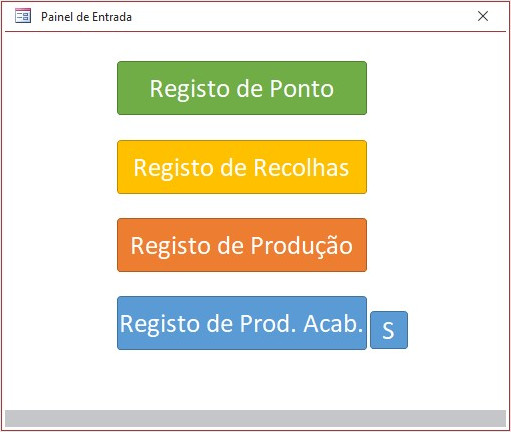
\includegraphics[width=\linewidth]{figuras/AppAccess/0-MenuInicial.jpg}
		\caption{Menu incial}
	\end{subfigure}
	\begin{subfigure}[c]{0.3\linewidth}
		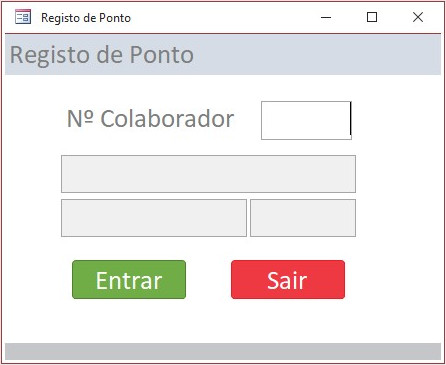
\includegraphics[width=\linewidth]{figuras/AppAccess/1-Ponto.jpg}
		\caption{Ecrã de marcação do ponto}
	\end{subfigure}
	\begin{subfigure}[c]{0.3\linewidth}
		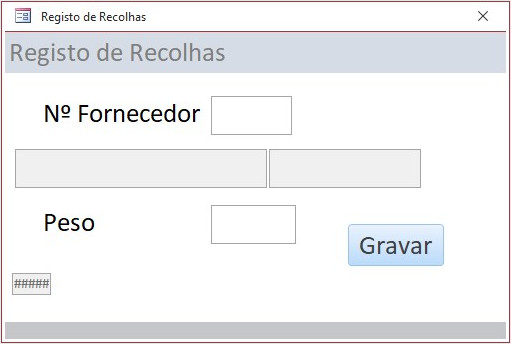
\includegraphics[width=\linewidth]{figuras/AppAccess/2-Recolha.jpg}
		\caption{Ecrã do registo de recolha}
	\end{subfigure}
	\begin{subfigure}[c]{0.3\linewidth}
		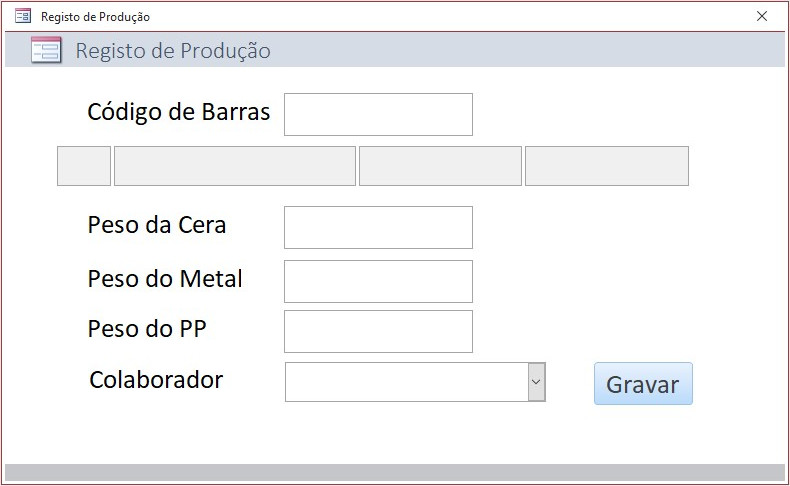
\includegraphics[width=\linewidth]{figuras/AppAccess/3-Producao.jpg}
		\caption{Ecrã do registo de produção}
	\end{subfigure}
	\begin{subfigure}[c]{0.3\linewidth}
		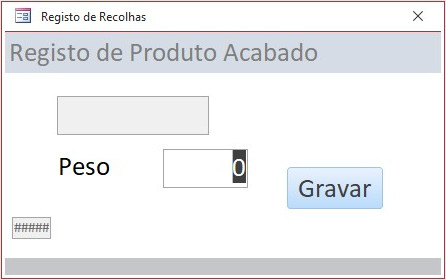
\includegraphics[width=\linewidth]{figuras/AppAccess/4-ProdutoAcabado.jpg}
		\caption{Ecrã do registo de produto acabado}
	\end{subfigure}
	\begin{subfigure}[c]{0.3\linewidth}
		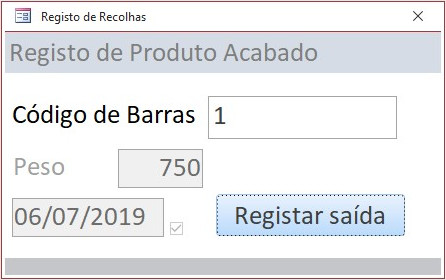
\includegraphics[width=\linewidth]{figuras/AppAccess/5-SaidaProdutoAcabado.jpg}
		\caption{Ecrã do registo de saída de produto acabado}
	\end{subfigure}
	
	\caption{Ecrãs da aplicação existe na empresa.}
	\label{fig:app_access}
\end{figure}

O fluxo dentro deste sistema era bastante simples. Ao executar o ficheiro Microsoft Access, era apresentado diretamente o menu ao utilizador. Este selecionaria a opção referente ao registo que pretendia fazer e uma nova janela surgia com o formulário correspondente. O utilizador preenchia com os dados requeridos e pressionava o botão "Gravar". Em caso de sucesso não era apresentado nenhuma mensagem. Em caso de erro era apresentada uma mensagem com essa informação. Estas mensagens era geradas diretamente pelo sistema de gestão de base de dados e não eram intuitivas. No caso de ser o registo de recolha ou de produto acabado, era ainda apresentado, numa nova janela um código de barras que seria impresso para identificar on elemento registado. Um exemplo do resultado impresso é demonstrado na figura \ref{fig:app_access_cb}.

\begin{figure}[H]
	\centering
	
	\begin{subfigure}[t]{0.4\linewidth}
		
\includegraphics[width=\linewidth]{figuras/AppAccess/2-CodBarras.jpg}
		\label{fig:app_access_cb_recolha}
		\caption{Recolha}
	\end{subfigure}
	\begin{subfigure}[t]{0.4\linewidth}
		
\includegraphics[width=\linewidth]{figuras/AppAccess/5-CodBarras.jpg}
		\label{fig:app_access_cb_prod_acabado}
		\caption{Produto Acabado}
	\end{subfigure}
	
	\caption{Exemplo dos códigos de barras gerados}
	\label{fig:app_access_cb}
\end{figure}
\noindent
Estes códigos de barras deveriam ter estruturas diferentes. O código de barras referente à recolha (figura \ref{fig:app_access_cb} (a) deveria ser constituído pelo código de barras correspondente ao ID da recolha, o ID do ponto de recolha e a data da recolha. Já no caso produto acabado era apenas apresentado o código de barras referente ao ID do mesmo (figura \ref{fig:app_access_cb} (b). A pedido da administração deveria passar a ser apresentado também o ID do produto acabado em formato numérico.\\
Após o estudo da aplicação foi iniciado o estudo da base de dados. Este estudo consistiu em compreender as tabelas que constituem base de dados, as suas relações e a informação que nelas era registada. Foi também solicitado pela empresa sugestões de melhoria do \textit{design} da base de dados com foco na coerência da informação registada.

\section{Modo de implementação do projeto}
Numa das reuniões discutiu-se o modo como o novo sistema deveria ser implementado. No dia em que ocorresse a primeira implementação do novo sistema, este deveria substituir por completo a aplicação construída no Microsoft Access. Isto porque devido à natureza da informação registada e tendo em conta que a base de dados teria a sua estrutura modificada, não era possível existir um período hibrido onde as duas aplicações coexistiram. Assim ficou definido que enquanto o novo sistema não fosse capaz de registar o ponto dos colaboradores, as recolhas efetuadas, as produções feitas, o produtos finalizados e a sua saída, a implementação não iria ocorrer.
Foi definido então que o sistema teria de passar por dois níveis de testes sendo o primeiro os testes de desenvolvimento e o segundo o teste com utilizadores reais de forma a identificar erros não previstos no período de desenvolvimento.

\section{Último levantamento de requisito}
Todos os requisitos da aplicação ficaram definidos no final da primeira semana, à excepção dos requisitos referentes a uma nova funcionalidade que permitisse o incremento do peso de uma recolha. Em algumas recolhas efetuada, o peso total da recolha superava a capacidade de ser pesado de uma só vez, seja pelo peso de matéria prima seja pela quantidade. Apesar de estarmos conscientes desta necessidade foi sugerido deixar a discussão sobre esta nova funcionalidade para o pós primeira implementação. Não se tratava de uma funcionalidade fundamental para o sistema e como tal havia a intenção de estudar a melhor forma de implementar esta solução e que apenas foi discutida na oitava semana do período de estágio. Consistiu na criação de uma nova tabela "Completar Recolha" que iria armazenar o histórico de incrementos feitos numa recolha, para assim poder identificar eventuais erros no registos da informação. Do ponto de vista da aplicação a recolha a ser incrementada seria identificada pelo código de barras impresso anteriormente e deveria ser apresentado ao utilizador o histórico de incrementos referente a essa recolha. Por fim definiu-se que uma recolha registada com o peso de zero quilos deveria redirecionar automaticamente o utilizador para o ecrã do incremento desta recolha após a impressão do primeiro código de barras.

\section{Lista final de requisitos}
Após as todas as reuniões de levantamento de requisitos, chegou-se à seguinte lista composta apenas por requisitos absolutos.
\begin{itemize}
	\item A aplicação só poderia ser acessível da rede interna
	\item A aplicação alojada num servidor físico com Ubuntu Server 18.04
	\item A aplicação WEB desenvolvida em PHP, com o framework Laravel, e em JavaScript;
	\item A aplicação teria de seguir o modelo \textit{Model View Controller} (MVC\label{sym:MVC});
	\item A aplicação deve ser construída de forma modular de forma a facilitar a sua manutenção no futuro;
	\item Uso de uma base de dados relacional, construída com o sistema de gestão de base de dados Microsoft SQL Server e a estrutura aprovada pela administração;
	\item A implementação teria de ser feita em duas fases:
	\begin{itemize}
		\item a primeira onde se substituía totalmente a aplicação existente na fabrica (Registo de ponto, de recolhas, de produção, de produto acabado e de saída de produto acabado);
		\item a segunda fase durante a qual as novas funcionalidades seriam aplicadas incrementalmente;
	\end{itemize}
	\item A aplicação teria de passar por uma fase de testes muito exigente para impedir erros que obrigassem ao uso da base de dados antiga.
	\item Os testes têm de ser divisos em dois níveis:
	\begin{itemize}
		\item Nível 1: testes de desenvolvimento;
		\item Nível 2: testes com utilizadores reais;
	\end{itemize}
	\item O sistema tem de ser graficamente coeso;
	\item O sistema terá de ter um tempo de aprendizagem mínimo no modo de utilização dos funcionários;
	\item O sistema deverá emitir mensagens após cada ação;
	\item As mensagens têm de ter linguagem simples e direta;
	\item O registo do horário de entrada e saída dos colaboradores;
	\item O registo do peso e ponto de recolha de onde vinha a matéria prima;
	\item Impressão de um código de barras com o ID gerado para a recolha inserida, ID do ponto de recolha e data de recolha;
	\item O sistema deve permitir de incrementar o peso de uma recolha;
	\item Se a recolha fosse iniciada com 0 kg é iniciado automaticamente o processo de incremento do peso da recolha que acabou de ser registada;
	\item Após o incremento do peso deveria ser impresso uma segunda via do código de barras dessa mesma recolha;
	\item Registo do peso de cera, metal e plástico de uma produção, bem como o colaborador associado;
	\item Registo do peso do produto final acabado;
	\item Impressão de um código de barras com o ID gerado para a produto final acabado;
	\item Registo da saída de produto acabado e cliente a quem foi vendido;
	\item Impressão de uma segunda via dos códigos de barras já impressos referente a uma recolha ou um produto acabado;
	\item Zona protegida por ID e \textit{Password} para a consulta dos registos feitos;
	\item As tabelas apresentadas na interface da aplicação teriam de ser capazes de refletir alterações na estrutura das tabelas da base de dados;
	\item O sistema deve permitir listar, inserir, editar, apagar e emitir uma segunda via de código de barras de uma \textit{recolha};
	\item O sistema deve permitir listar, inserir, editar e apagar uma \textit{produção};
	\item O sistema deve permitir listar, inserir, editar, apagar e emitir uma segunda via de código de barras de um \textit{produto acabado};
	\item O sistema deve permitir listar, inserir, editar, apagar e desativar um \textit{colaborador};
	\item O sistema deve permitir listar, inserir, editar e apagar um \textit{registo de ponto};
	\item O sistema deve permitir listar, inserir, e apagar um \textit{utilizador};
	\item O sistema deve permitir listar, inserir e editar uma \textit{entidade};
	\item O sistema deve permitir listar, inserir, editar, apagar e desativar um \textit{ponto de recolha};
	\item O sistema deve permitir listar, inserir, editar, apagar e desativar um \textit{cliente};
	\item O sistema deve permitir listar, inserir, editar, apagar e executar uma \textit{analise personalizada};
	\item \textit{Script} de analise da coerência dos dados registados para Pontos de Recolha, Registos de Ponto e Produção.
\end{itemize}
\cleardoublepage
% ************ Chapter 4 ************
\chapter{Projeção do Sistema de Informação} 
\label{cap:4}
Levantados os requisitos do projeto, iniciou-se projeção do sistema. Este foi um processo que envolveu desde planeamento de trabalho a ser realizado, ao design da aplicação.

\section{Planeamento do projeto}
A primeira semana do período do estágio foram destinadas ao levantamento de requisitos. Foi ainda durante esta semana que ocorreu o redesign da base de dados.
As semanas 2 e 3 foram destinadas ao estudo dos \textit{frameworks} a utilizar, do sistema de gestão de base de dados e do ambiente da empresa.
Conforme indicado nos requisitos do projeto, o desenvolvimento do sistema de informação teria de ser dividido em duas fases. A data para a conclusão da primeira fase foi fixada no inicio da sexta semana, dando-se logo incio à fase dois.

\section{Design da nova base de dados}
A base de dados a ser utilizada neste projeto teve como ponto de partida aquela que já era utilizada pela aplicação antiga. De modo a tornar a estrutura o mais adequada possível, numa da reuniões, foi solicitado à administração que descrevesse em detalhe o fluxo de informação da estrutura até à data implementada. Após a reunião seguiu-se um estudo para encontrar formas de otimizar a estrutura da base de dados, não apenas na questão da normalização da estrutura mas também de forma a tornar o trabalho futuro mais simples procurando meios de otimizar o fluxo da informação. Após o estudo foi entregue de uma proposta da nova estrutura. Esta foi chumbada numa fase inicial porque, como resultado da normalização, foi criada uma tabela destinada a armazenar os cemitérios com os quais a empresa tem parceria, uma segunda tabela onde ficaram registadas as empresas a quem a Natural Life compra o materia-prima e uma terceira tabela responsável por agregar os registos das primeiras duas de modo a estabelecer as relações com a restantes tabelas do sistema. A reposta da administração foi que preferia que existisse apenas uma única tabela, que agregasse os campos das três referidas anteriormente, com um campo extra para distinguir o tipo de registo. Apesar de compreenderem qual era o intuito da mudança sugerida, esta iria tornar mais difícil a adaptação de ficheiros Excel e PowerBi já existentes. A mudança pedida foi efetuada e a administração aceitou as restantes alterações sugeridas. Dentre dela destaca-se a tabela "Entidades" criada para armazenar as informações de identificação (nome, morada, código postal e nif) dos pontos de recolha e clientes. Esta alteração permitiu não só reunir num único local a lista de entidades com as quais a Natural Life interage, eliminado eventuais incoerências de informação a respeito do numero de identificação fiscal, por exemplo.
O processo de reforma da base de dados manteve-se então congelado até à sétima semana, na qual se criou a tabela "completar\_recolha", conforme descrito no capítulo anterior. No final de todo este processo a estrutura final da base de dados, aprovada pela administração, é a descrita na figura \ref{fig:db_model}.

\begin{figure}[htbp] 
	\begin{center}
		% Requires \usepackage{graphicx}
		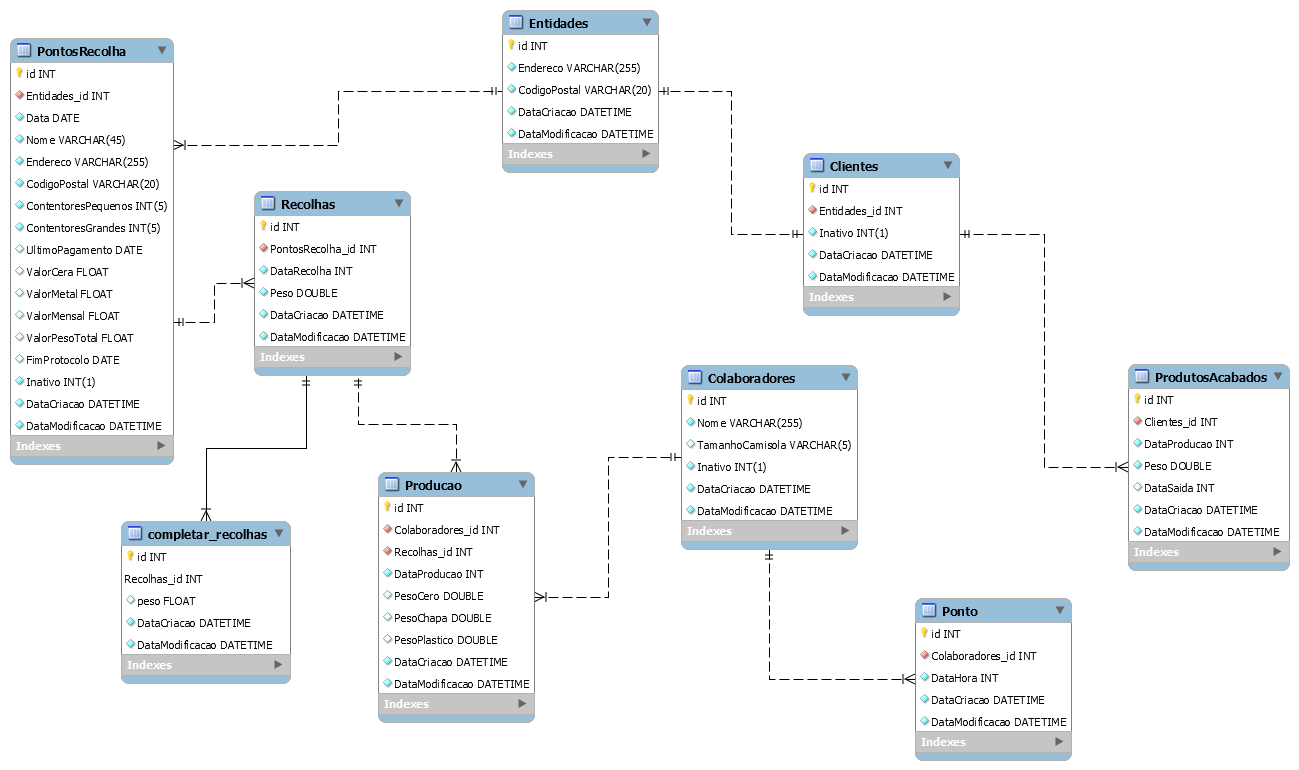
\includegraphics[width=\textwidth,keepaspectratio]{figuras/DB_Model/new.png}
		\caption{Estrutura final da base de dados}
		\label{fig:db_model} 
	\end{center}
\end{figure}

Finalizado este processo, iniciou-se o processo de design da aplicação.

\section{Aplicação}
Respondendo aos requisitos definidos no Capitulo \ref{cap:3}, a aplicação a ser desenvolvida seria uma aplicação web construída em PHP, com o framwork laravel, e JavaScript segundo o padrão do modelo MVC. O modelo MVC, representado na figura \ref{fig:mvc}, descreve a forma como uma aplicação deve ser construída separando-a em três camadas distintas: Model View e Controller. Esta separação server distinguir representações de informação internas dos modos como a informação é apresentada ao utilizador\cite{Wikipediad}.
Esta abstração em camadas é particularmente vantajosa no que toca a fazer reutilização de código, pois tendo em conta as regras do modelo cada classe tem apenas uma responsabilidade atribuída além de o projeto ter um baixo acoplamento entre si. Desta forma é muito fácil utilizar a mesma classe partes distas do projeto, facilitando a sua compreensão, manutenção e atualização.
Estas características do modelo servem ainda de resposta a outros requisitos do projeto como modularidade do projeto.
\begin{figure}[H] 
	\begin{center}
		% Requires \usepackage{graphicx}
		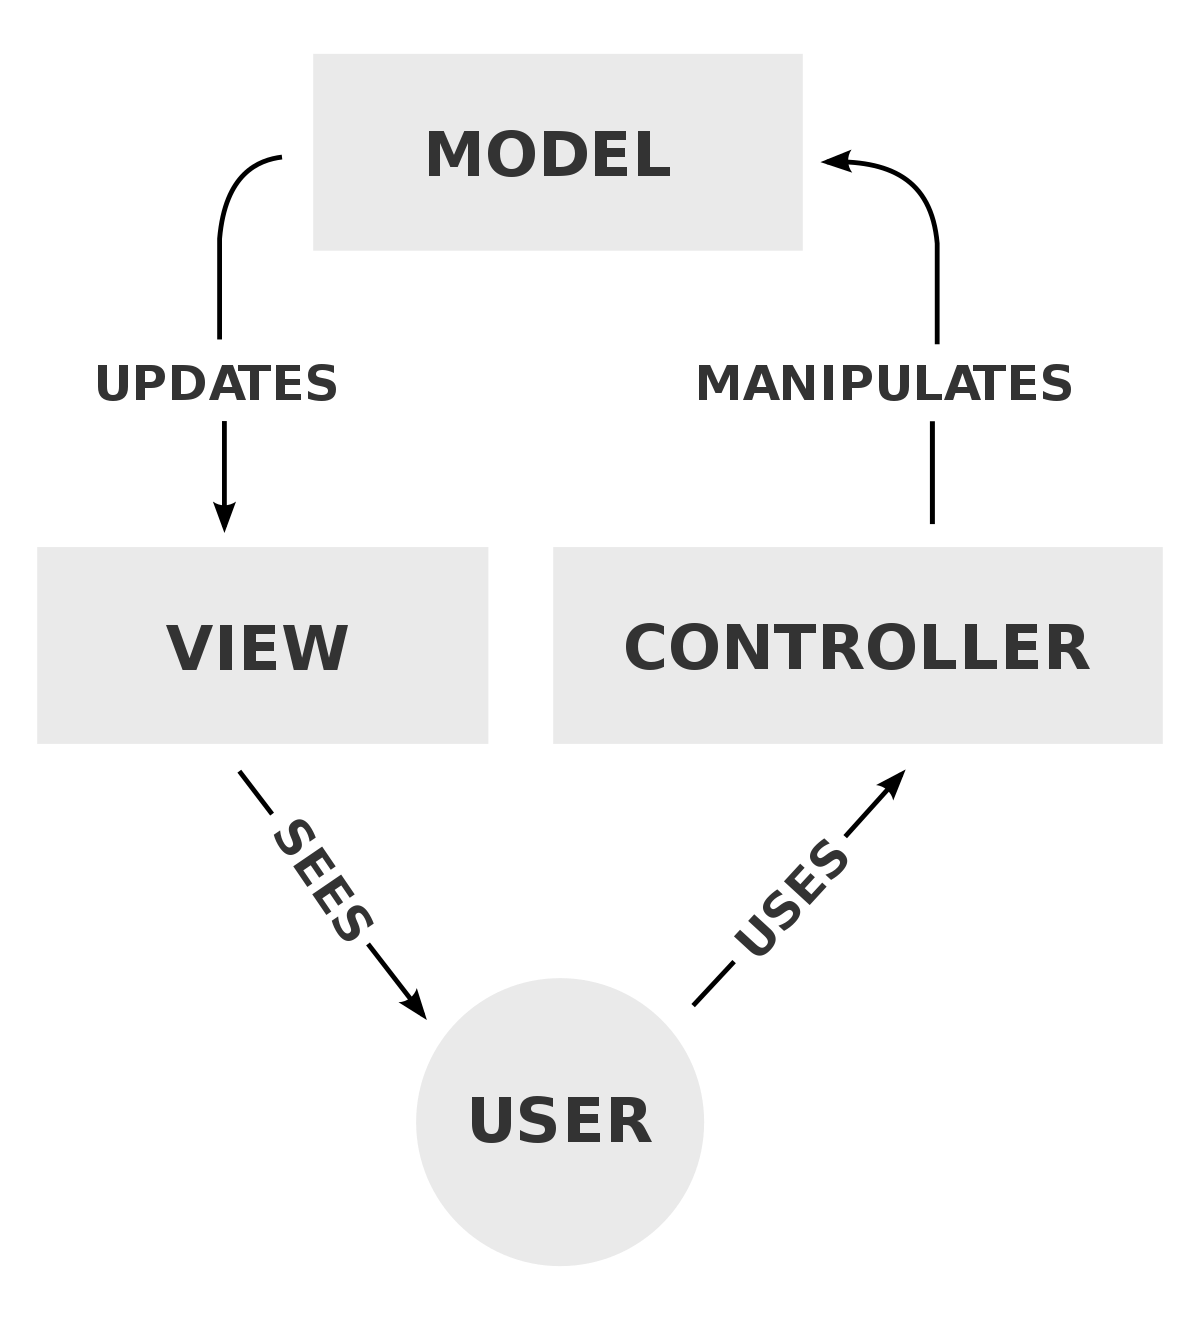
\includegraphics[width=0.30\textwidth,keepaspectratio]{figuras/mvc.png}
		\caption{Diagrama do modelo MVC}
		\label{fig:mvc} 
	\end{center}
\end{figure}

\noindent 
Ainda respondendo aos requisitos deveria existir duas áreas distintas dentro da aplicação destinada aos colaboradores na fábrica e à administração.
Estas suas sub-aplicações foram designadas de Aplicação Fábrica, acessível aos colaboradores da empresa e responsável pelos registos de informação na base de dados, e a Aplicação Painel, protegida por um sistema de autenticação na qual seria possível manipular toda a informação registada.
Para fazer esta separação, os endereços dentro da aplicação foram divididos em dois grupos distintos. Em primeiro lugar as páginas associadas à Aplicação de Fábrica estavam sob o endereço /Fabrica:

\begin{center}
\url{http://<ip.do.servidor>/Fabrica/<Nome_da_página_solicitada>}
\end{center}

\noindent 
Enquanto as páginas relacionadas com a Aplicação Painel estavam sob o endereço /Painel:

\begin{center}
	\url{http://<ip.do.servidor>/Painel/<Nome_da_página_solicitada>}
\end{center}

\noindent 
A única exceção a esta regra está no diretório raiz do sistema, que direciona para a página index da Aplicação de Fábrica.\\
Esta organização em nada muda a estrutura de ficheiros do projeto. O framework laravel, trás consigo um recurso de rotas, que permite facilmente que este tipo de regras seja incluída no projeto sem ter necessariamente que fazer modificações à árvore de diretórios da aplicação. Desta forma, manteve-se uma estrutura dos ficheiros da aplicação coesa, mantendo cada tipo de ficheiro na sua pasta definida e manter regras de padronização dos endereços da aplicação.

\section{Casos de uso do sistema}
Definidos todos os detalhes supracitados, é possível dar inicio à definição de cada um dos casos de uso do projeto. Esta definição serve como guia de desenvolvimento, mantendo as informações necessárias para se conhecer o comportamento esperado de cada um dos casos de uso do sistema final e é explicada nas próximas páginas.
\newpage

% Aplicação Fábrica
\subsection{Aplicação Fábrica: Menu Inicial}
\subsubsection*{Descrição do caso de uso}
No menu, espera-se que este seja muito simples e intuitivo. Deve conter botões que indiquem de forma inequívoca qual a qual funcionalidade dão acesso. As cores das opções já existentes na aplicação construida no Microsoft Access deverão ter cores similares.\\
Na primeira fase do projeto este menu deve apenas contemplar as opções existentes na aplicação anterior, tal como descrito na figura \ref{fig:di_fabrica_menu} a.\\
No final da segunda fase, espera-se que o menu inicial apenas acrescente dois botões no final, conforme demonstrado na figura \ref{fig:di_fabrica_menu} b

\begin{figure}[H]
	\centering
	
	\begin{subfigure}[t]{0.45\linewidth}
		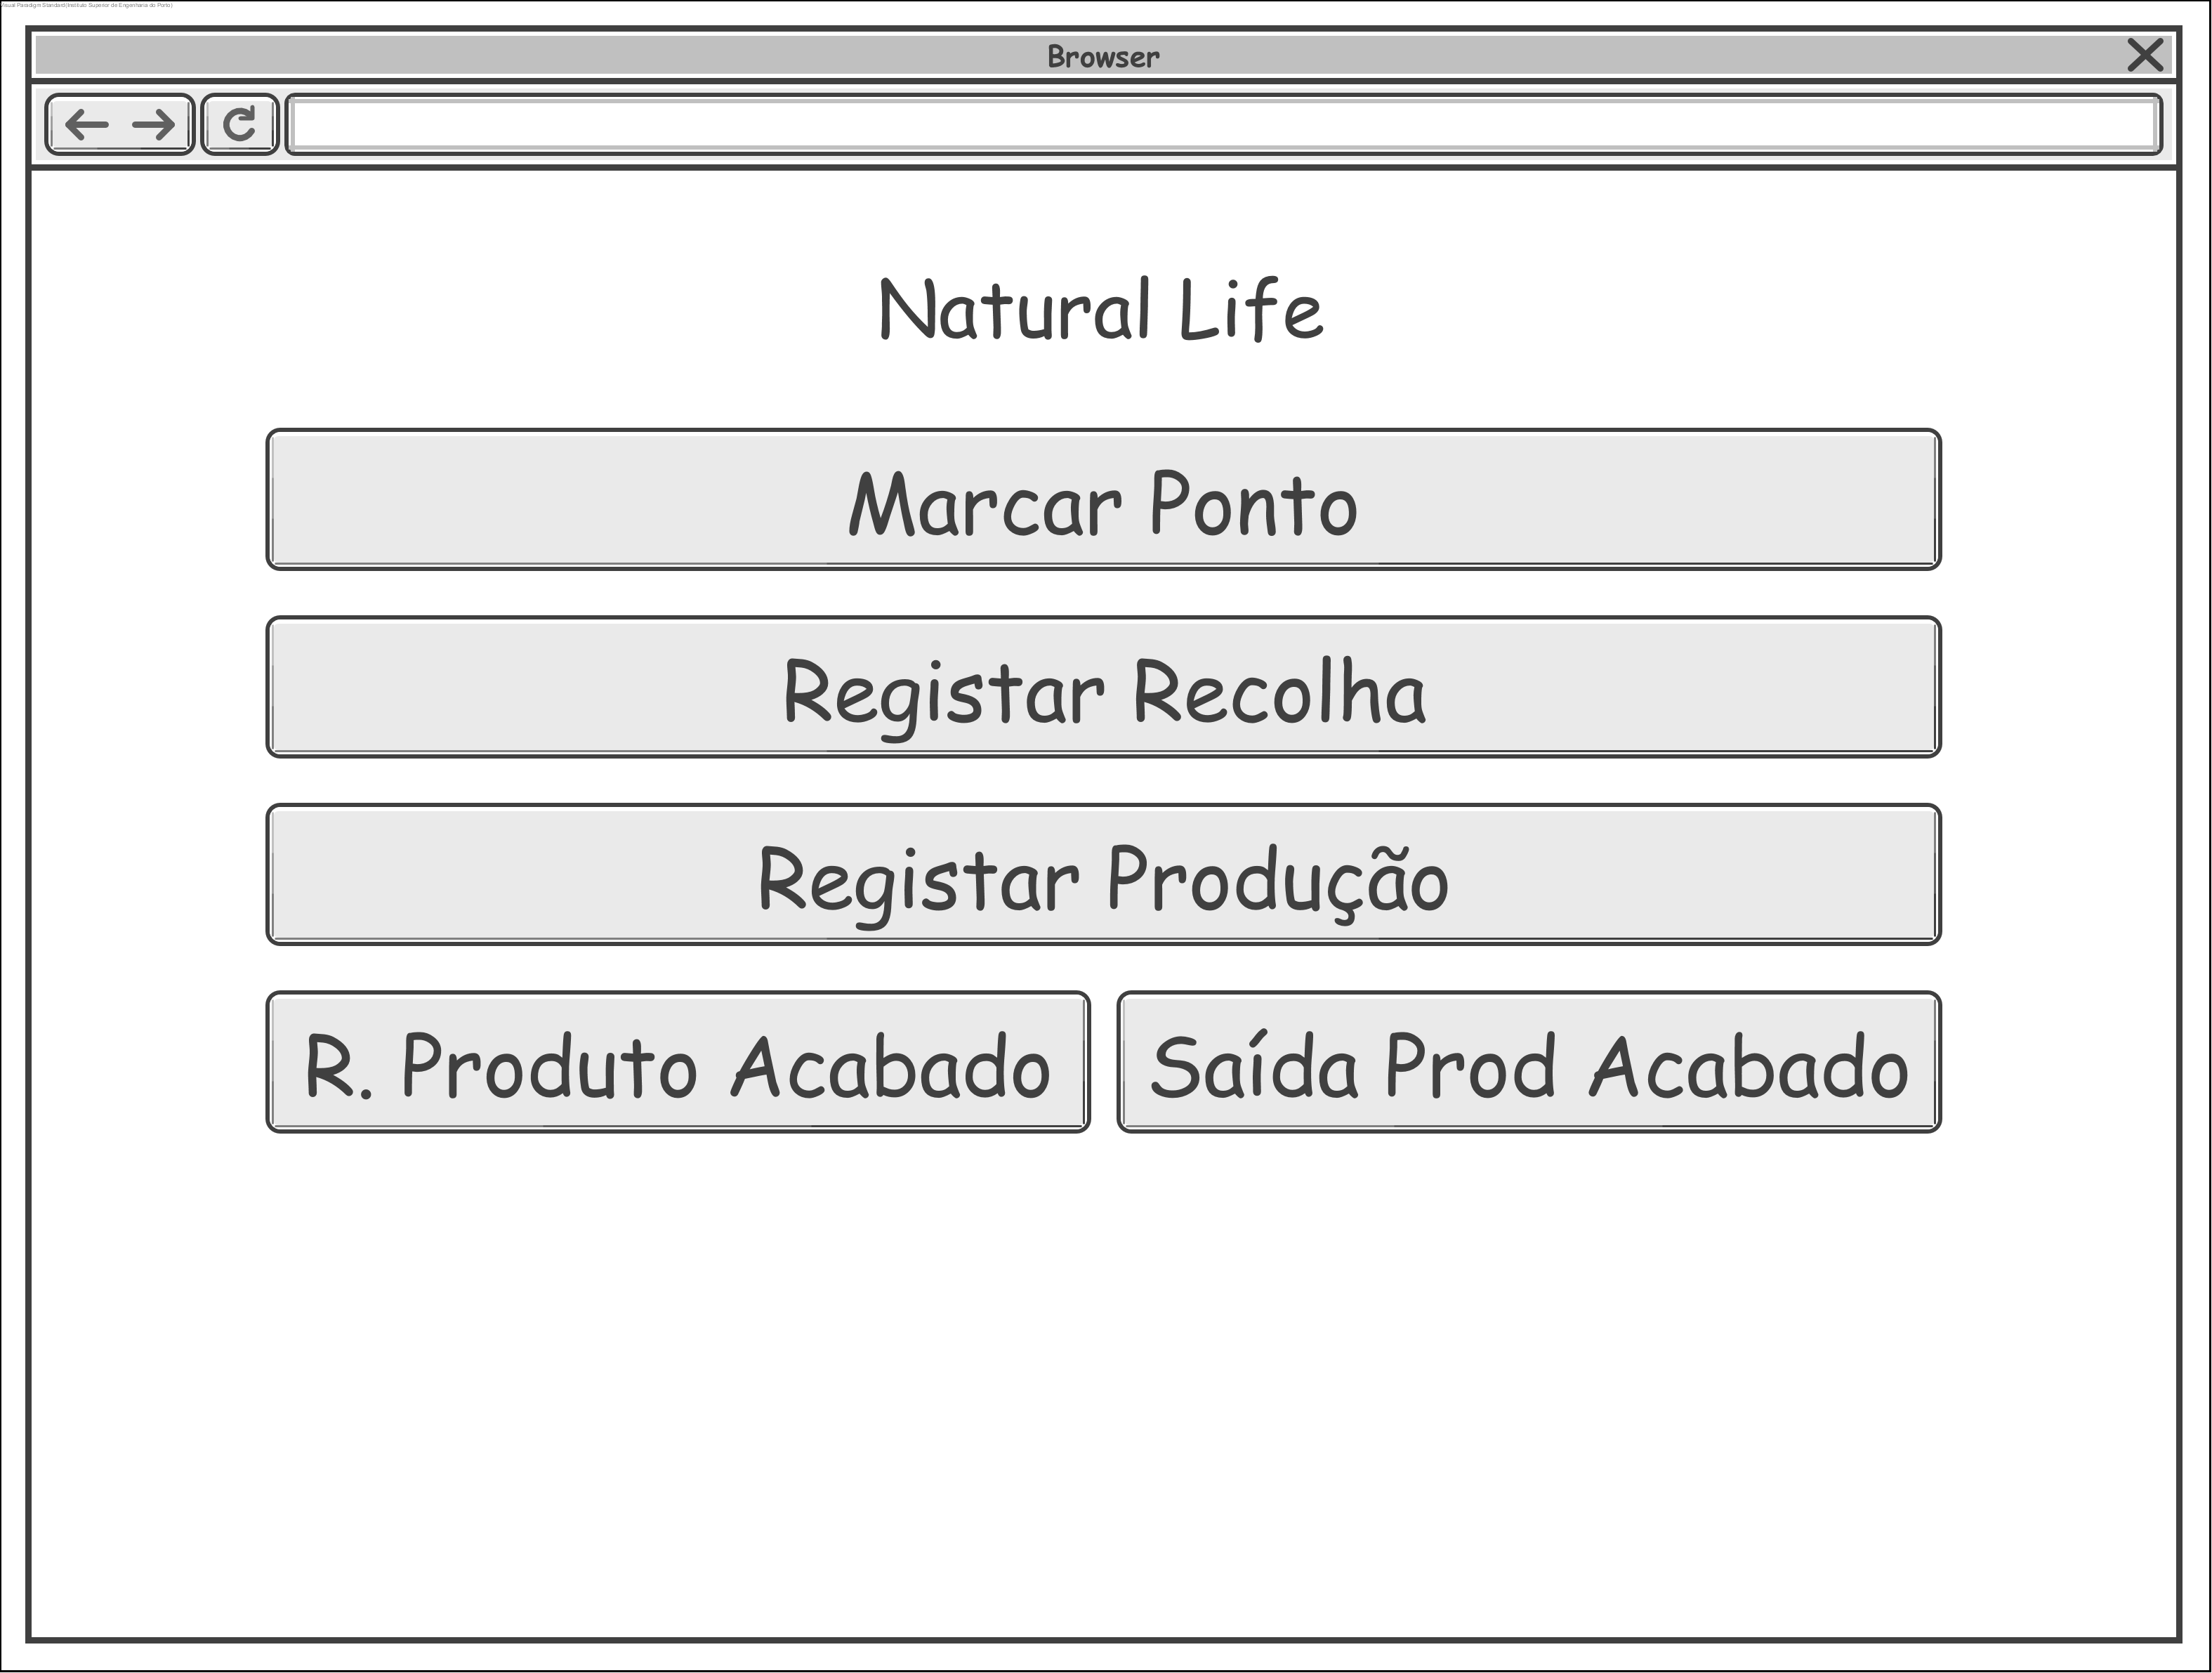
\includegraphics[width=\linewidth]{figuras/Diagramas_vp/DI_Fabrica_0-Menu_Inicial_-1a_Fase.png}
		\label{fig:di_fabrica_menu_1}
		\caption{Após concluir primeira fase}
	\end{subfigure}
	\begin{subfigure}[t]{0.45\linewidth}
		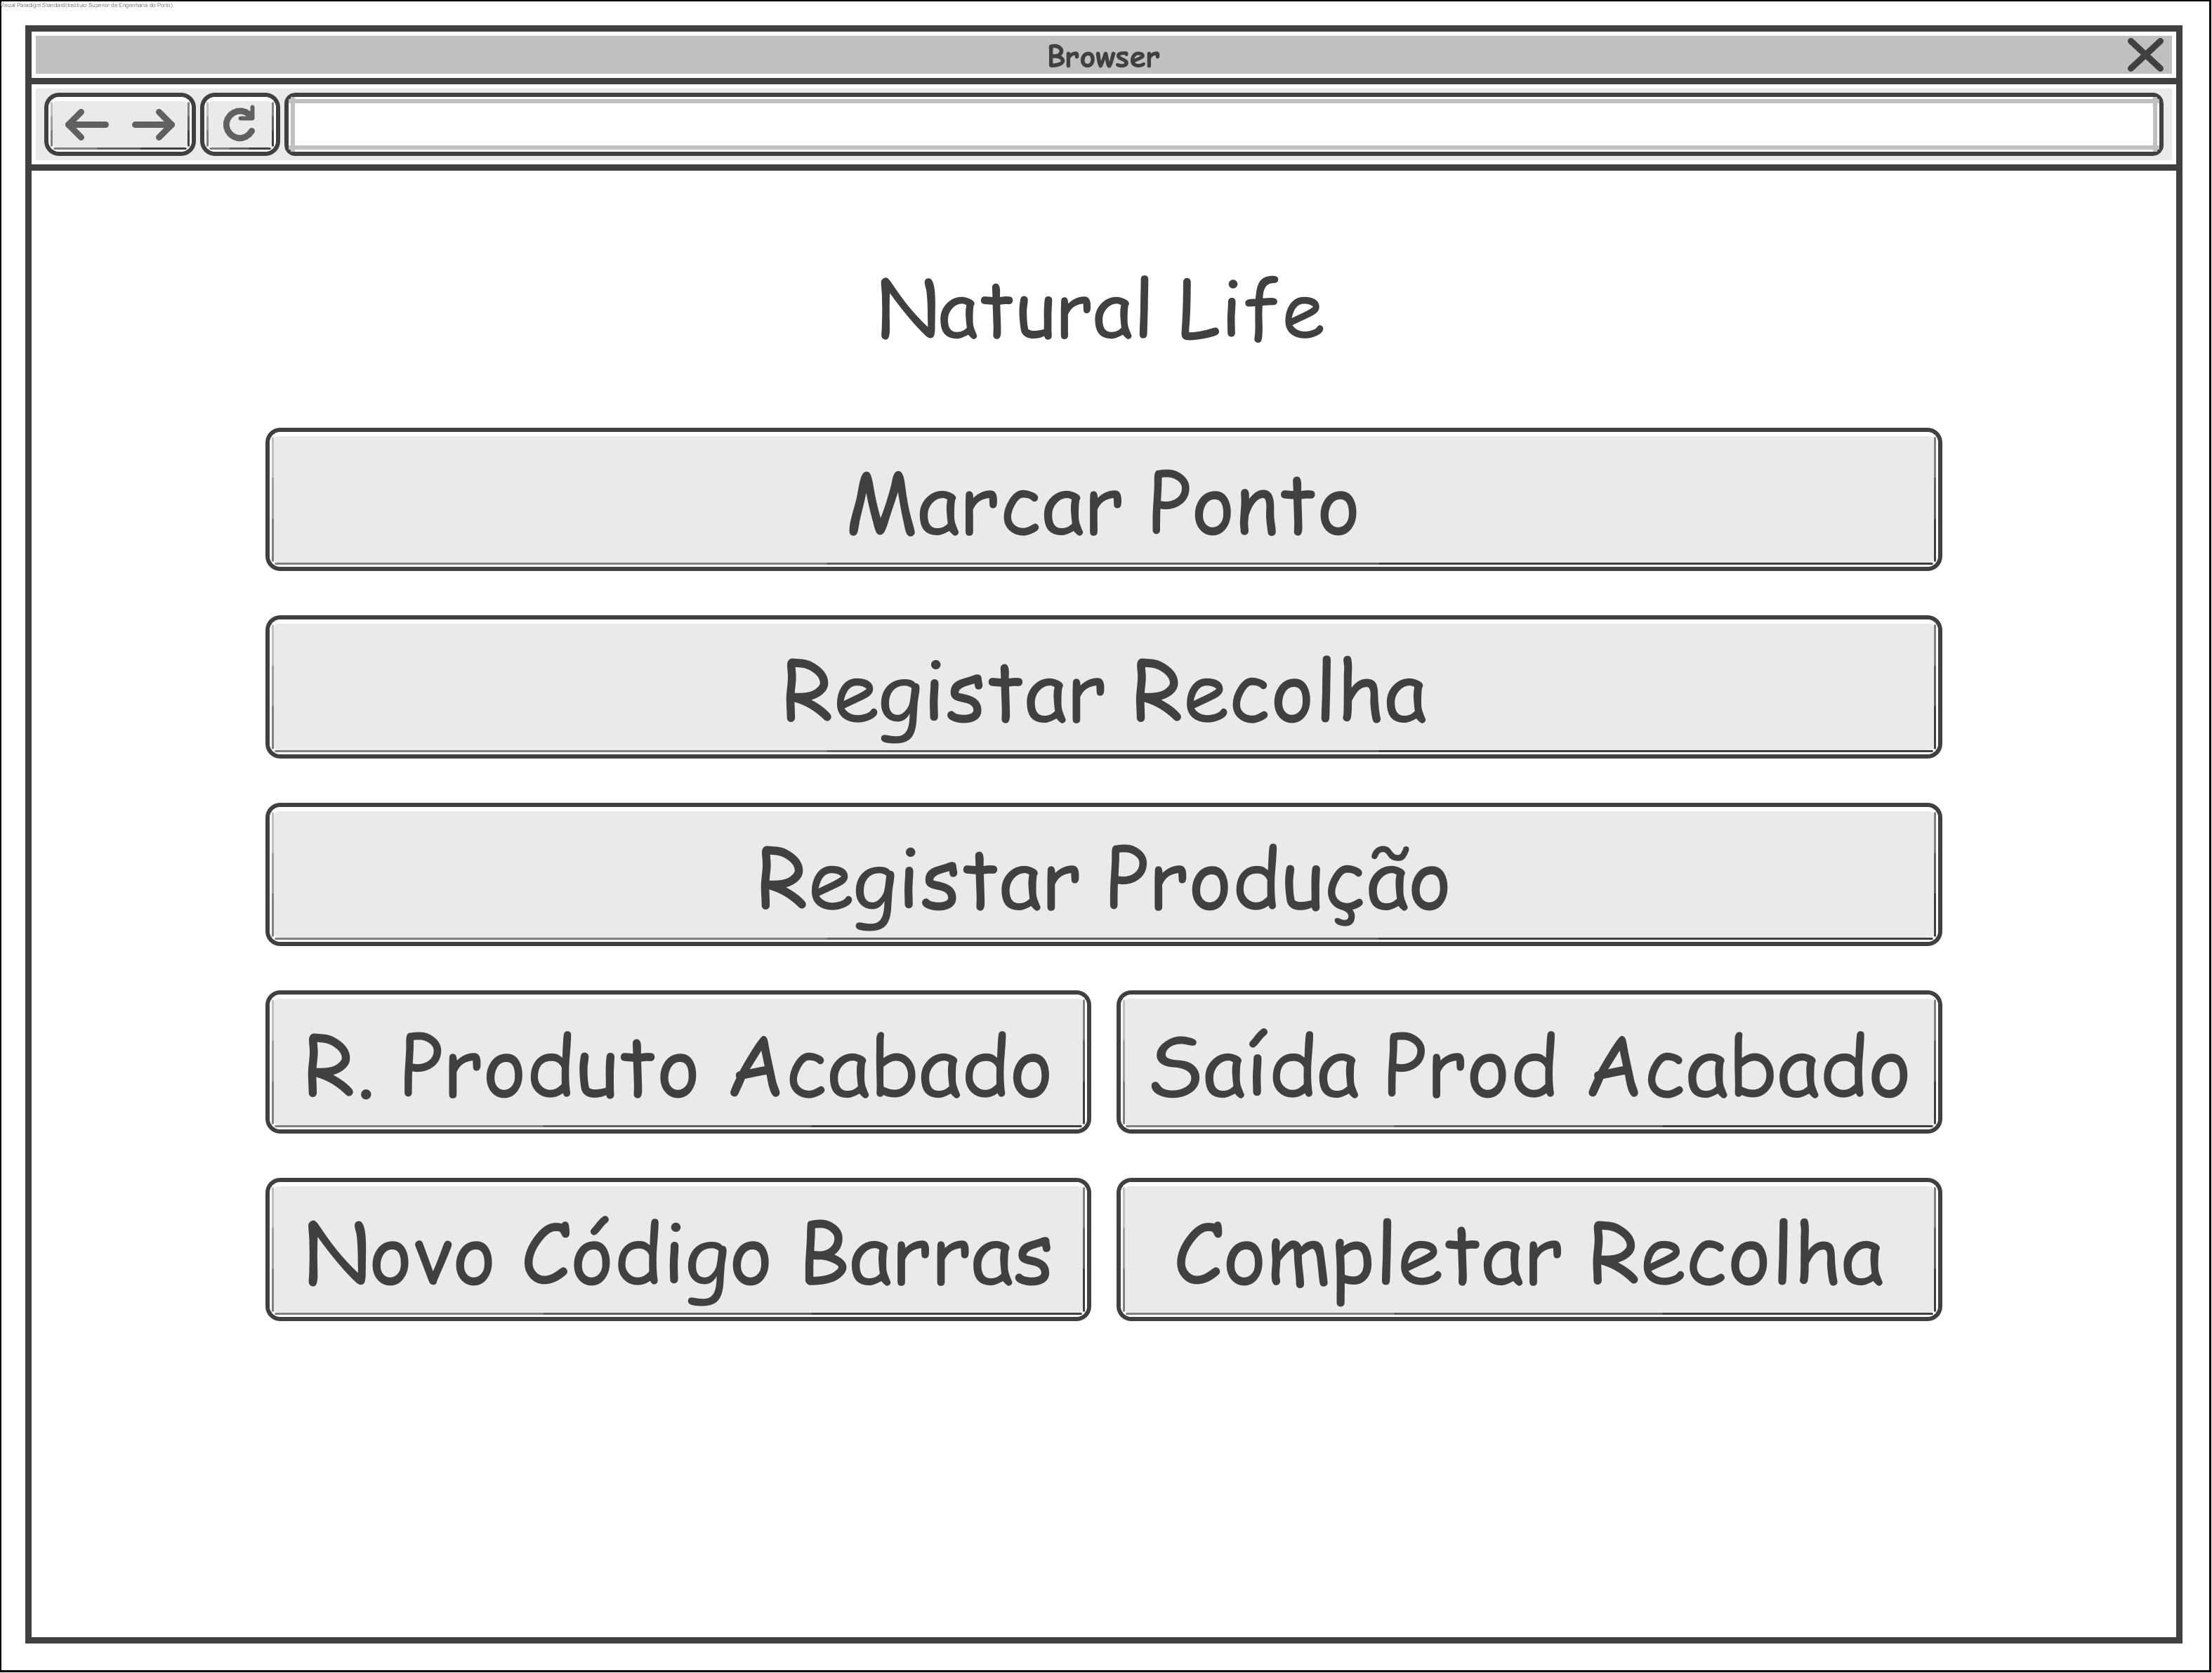
\includegraphics[width=\linewidth]{figuras/Diagramas_vp/DI_Fabrica_0-Menu_Inicial_-2a_Fase.png}
		\label{fig:di_fabrica_menu_2}
		\caption{Após concluir segunda fase}
	\end{subfigure}
	
	\caption{Modelo do menu}
	\label{fig:di_fabrica_menu}
\end{figure}
\newpage
\subsection{Aplicação Fábrica: Registo de Ponto}
\subsubsection*{Descrição do caso de uso}
No registo do ponto, espera-se que utilizador entre na página e indique apenas o seu ID. A informação sobre a data e hora do registo deve ser automaticamente definida pelo sistema. 

\begin{figure}[H] 
	\begin{center}
		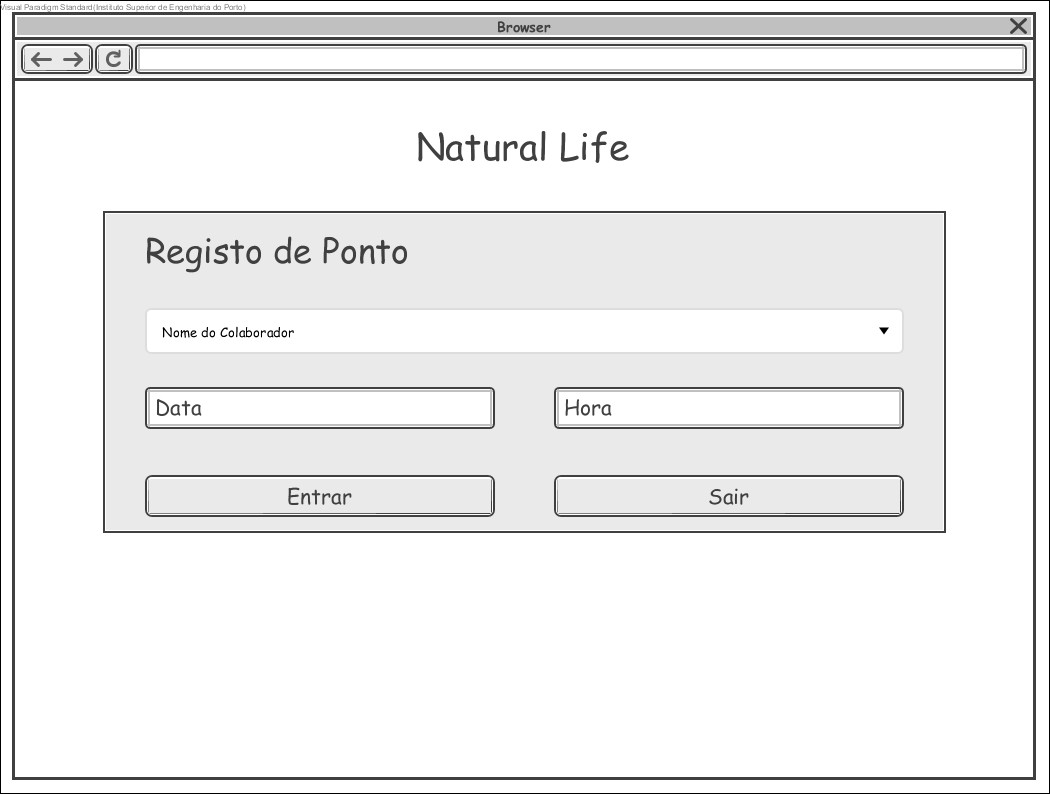
\includegraphics[width=0.60\textwidth,keepaspectratio]{figuras/Diagramas_vp/DI_Fabrica_1_Marcar_Ponto.jpg}
		\caption{Modelo do formulário do registo do ponto}
		\label{fig:di_ponto} 
	\end{center}
\end{figure}

\subsubsection*{Fluxo do caso de uso}
O caso de uso inicia-se com a abertura da página do registo de ponto. É apresentado o formulário com a data e hora previamente preenchidas. O utilizador tem de indicar o seu ID numa lista de dropdown. Após indicar o seu ID precisona o botão "Entrada" ou "Saída" conforme se esta a indicar o horario de entrada ou saída, respetivamente. Ambos os botões executam a submissão do formulário. Após o registo é apresentada uma mensagem ao utilizador


\begin{figure}[H] 
	\begin{center}
		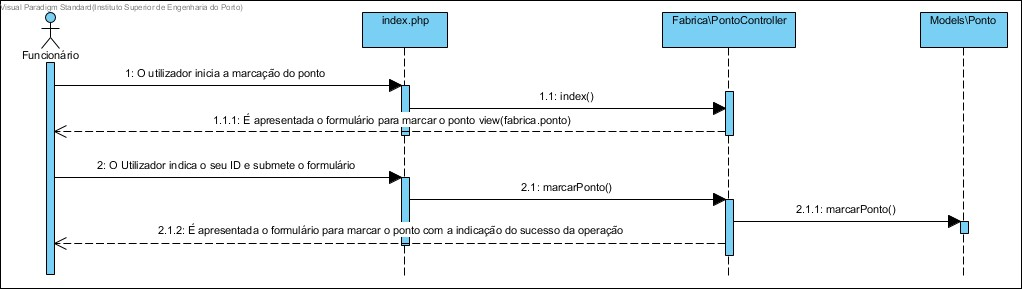
\includegraphics[width=\textwidth,keepaspectratio]{figuras/Diagramas_vp/SD_Fabrica_1_Marcar_Ponto.jpg}
		\caption{Diagrama de sequência marcar ponto}
		\label{fig:sd_ponto} 
	\end{center}
\end{figure}
\newpage
\subsection{Aplicação Fábrica - Registo de recolha}
\subsubsection*{Descrição do caso de uso}
No registo de recolha, espera-se que utilizador entre na página e indique o ID do ponto de recolha e o peso da recolha. A informação da data deve ser indicada automaticamente pelo sistema. A aparência da \textit{view} deste caso de utilização será semelhante ao demonstrado na figura \ref{fig:di_recolha}. 

\begin{figure}[H] 
	\begin{center}
		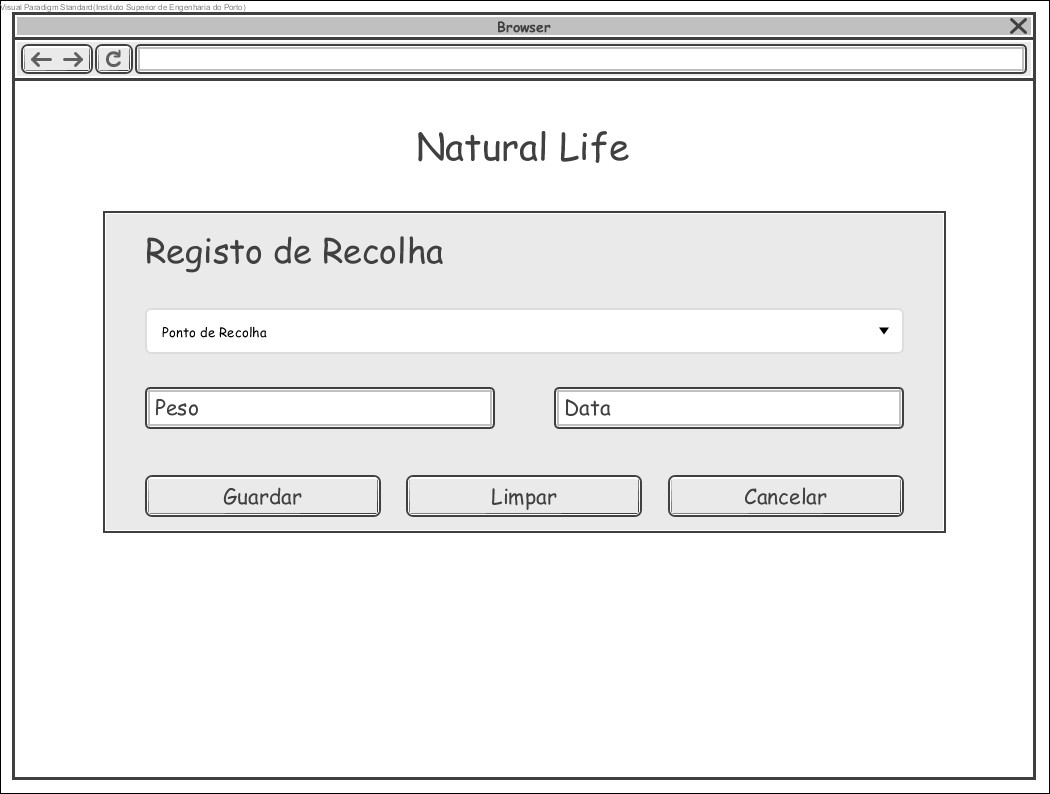
\includegraphics[width=0.60\textwidth,keepaspectratio]{figuras/Diagramas_vp/DI_Fabrica_2_Registo_de_Recolha.jpg}
		\caption{Modelo do formulário do registo de recolha}
		\label{fig:di_recolha} 
	\end{center}
\end{figure}

\subsubsection*{Fluxo do caso de utilização}
O caso de uso inicia-se com a abertura da página do registo de recolha. É apresentado o formulário com a data previamente preenchida. O utilizador tem de indicar o ID do ponto de recolha numa lista de \textit{dropdown} e o peso da recolha feita. Após indicar as informações solicitadas precisona o botão \textit{Guardar}. No final do registo é apresentada uma mensagem ao utilizador. Caso o registo seja feito com sucesso um novo separador é aberto com o código de barras para ser impresso, tal como demonstrado na figura \ref{fig:sd_recolha}.


\begin{figure}[H] 
	\begin{center}
		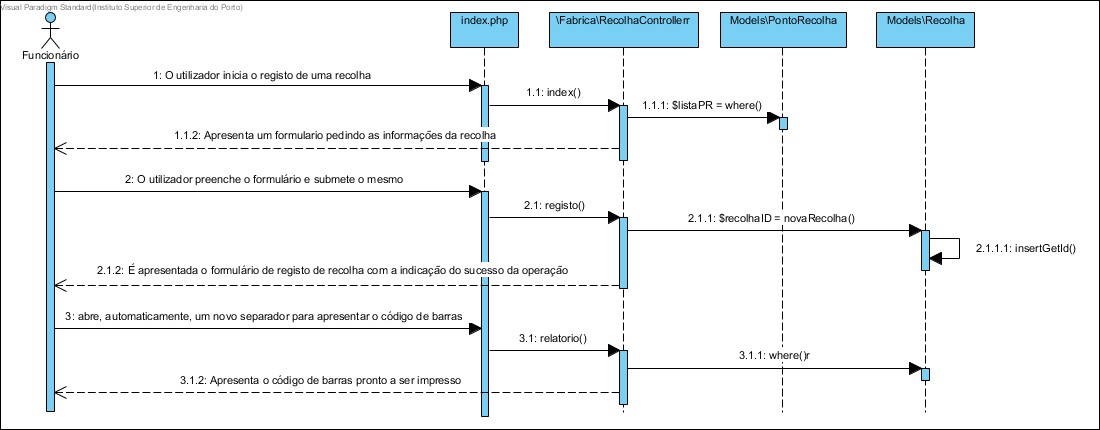
\includegraphics[width=\textwidth,keepaspectratio]{figuras/Diagramas_vp/SD_Fabrica_2_Registo_de_Recolhas.jpg}
		\caption{Diagrama de sequência registo de recolha}
		\label{fig:sd_recolha} 
	\end{center}
\end{figure}
\newpage
\subsection{Aplicação Fábrica: Produção}
\subsubsection*{Descrição do caso de uso}
No registo de produção, espera-se que utilizador entre na página e indique o código de barras da recolha, o peso de cera, metal e plástico e o seu ID. A informação da data de produção deve ser indicada automaticamente pelo sistema e a informação sobre a recolha (ponto de recolha e data da recolha) seja obtido, em background, após indicar o código de barras da recolha.

%\begin{figure}[H] 
%	\begin{center}
%		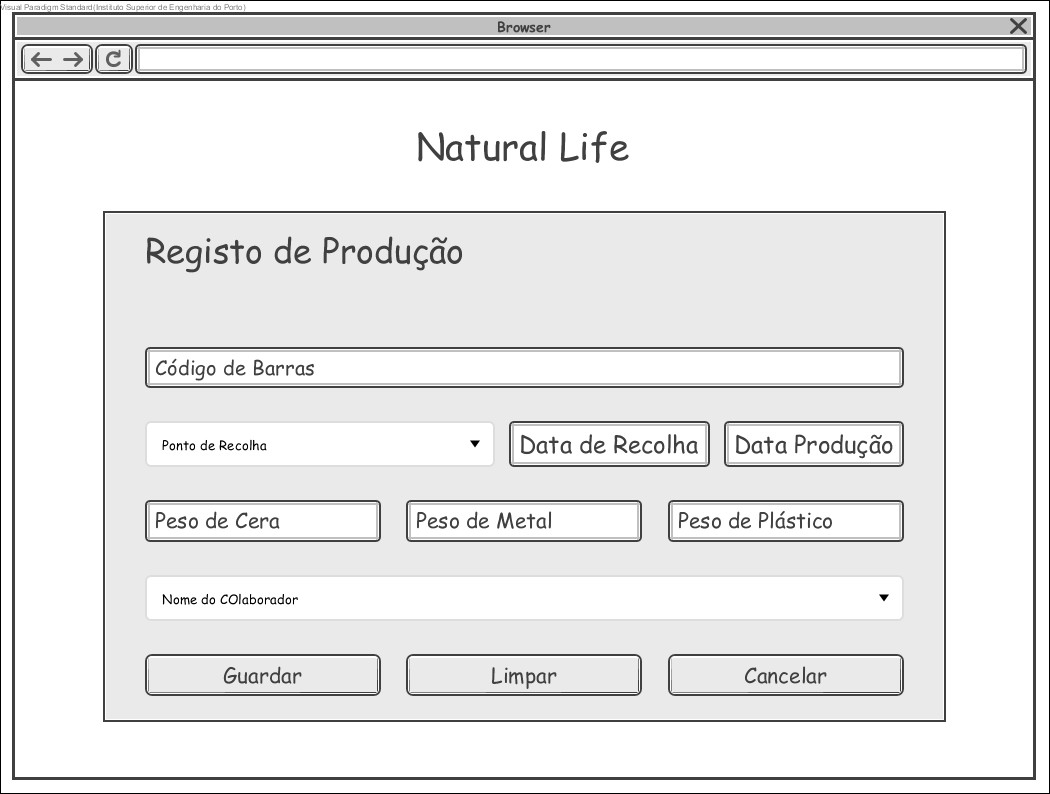
\includegraphics[width=0.60\textwidth,keepaspectratio]{figuras/Diagramas_vp/DI_Fabrica_3_Registo_de_Produção.jpg}
%		\caption{Modelo do formulário do registo de produção}
%		\label{fig:di_producao} 
%	\end{center}
%\end{figure}
\todo{falta os diagramas}

\subsubsection*{Fluxo do caso de uso}
O caso de uso inicia-se com a abertura da página do registo de produção. É apresentado o formulário com a data de produção previamente preenchida. O utilizador tem de indicar o código de barras da recolha, peso de cera, metal e plástico e o seu ID numa lista de dropdown. Quando o utilizador termina de indicar o código da recolha é feito um request ao servidor para saber o ponto de recolha e data da recolha. Essa informação é apresentada automaticamente ao utilizador Após indicar as informações solicitadas precisona o botão "Guardar". No final do registo é apresentada uma mensagem ao utilizador.

%\begin{figure}[H] 
%	\begin{center}
%		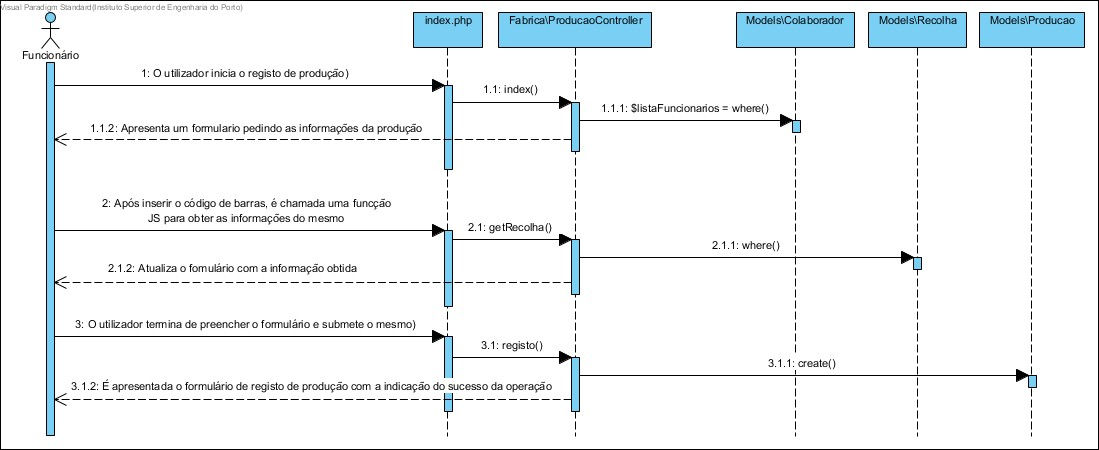
\includegraphics[width=\textwidth,keepaspectratio]{figuras/Diagramas_vp/SD_Fabrica_3_Registo_de_Produção.jpg}
%		\caption{Diagrama de Sequência registo de produção}
%		\label{fig:sd_producao} 
%	\end{center}
%\end{figure}
\todo{falta os diagramas}
\newpage
\subsection{Aplicação Fábrica: Registo de Produto Acabado}
\subsubsection*{Descrição do caso de uso}
No registo de produto acabado, espera-se que utilizador entre na página e indique o peso do produto acabado. A informação da data deve ser indicada automaticamente pelo sistema. 

\begin{figure}[H] 
	\begin{center}
		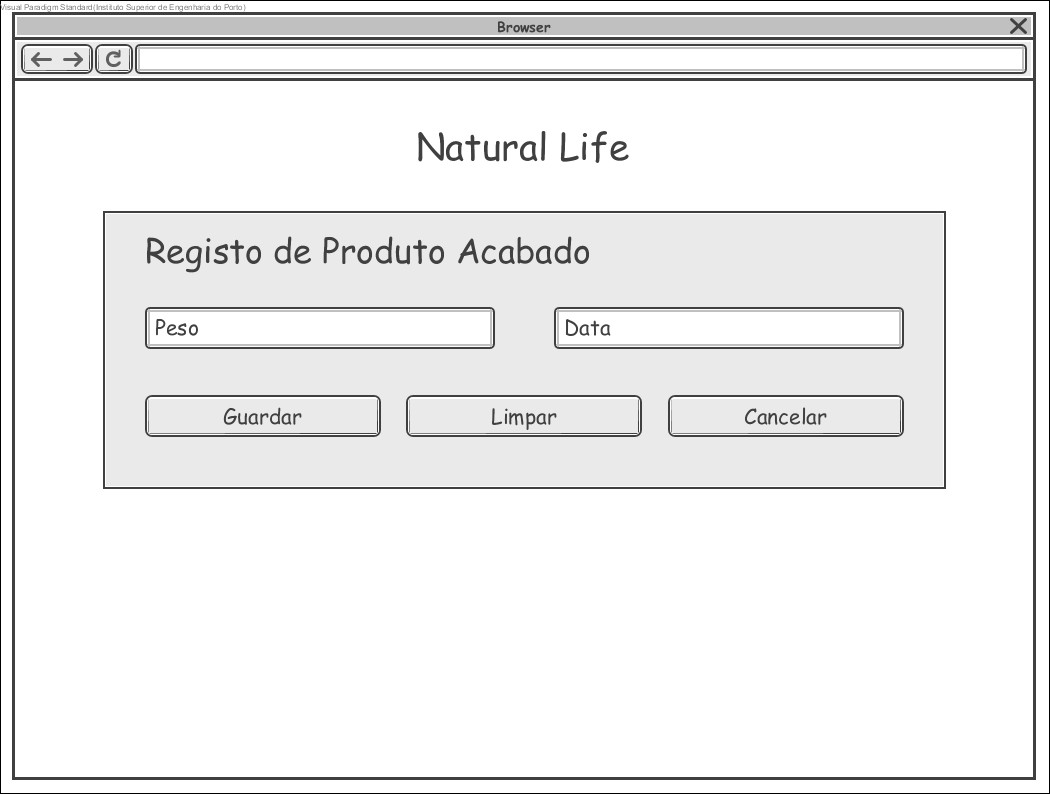
\includegraphics[width=0.60\textwidth,keepaspectratio]{figuras/Diagramas_vp/DI_Fabrica_4_Registo_de_Produto_Acabado.jpg}
		\caption{Modelo do formulário do registo de produto acabado}
		\label{fig:di_prod_acabado} 
	\end{center}
\end{figure}

\subsubsection*{Fluxo do caso de uso}
O caso de uso inicia-se com a abertura da página do registo de produto acabado. É apresentado o formulário com a data previamente preenchida. O utilizador tem de indicar o peso do produto acabado. Após indicar as informações solicitadas precisona o botão "Guardar". No final do registo é apresentada uma mensagem ao utilizador. Caso o registo seja feito com sucesso um novo separador é aberto com o código de barras para ser impresso.


\begin{figure}[H] 
	\begin{center}
		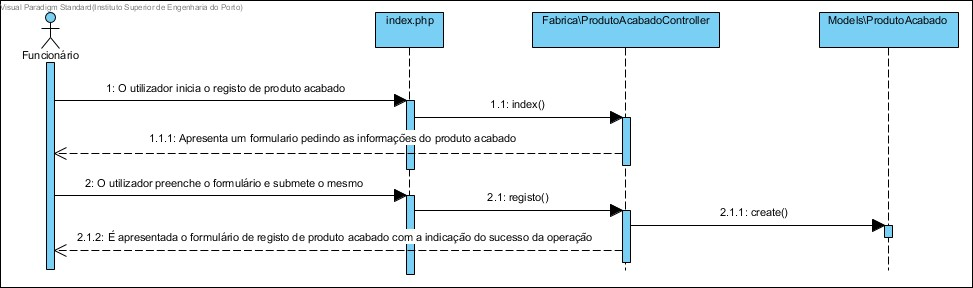
\includegraphics[width=\textwidth,keepaspectratio]{figuras/Diagramas_vp/SD_Fabrica_4_Registo_de_Produto_Acabado.jpg}
		\caption{Diagrama de sequência registo de produto acabado}
		\label{fig:sd_prod_acabado} 
	\end{center}
\end{figure}
\newpage
\subsection{Aplicação Fábrica - Registo de Saída de Produto Acabado}
\subsubsection*{Descrição do caso de uso}
No registo de produto acabado, espera-se que utilizador entre na página e indique o código de barras do produto acabado. A informação da data deve ser indicada automaticamente pelo sistema. A partir da segunda fase do projeto deverá ainda existir um campo para indicar o cliente. A aparência da \textit{view} deste caso de utilização será semelhante ao demonstrado na figura \ref{fig:di_saida_prod_acabado}. A figura  \ref{fig:di_saida_prod_acabado} (a) descreve como será a interface após concluir a primeira fase do projeto e a figura  \ref{fig:di_saida_prod_acabado} (b) descreve como será a interface após concluir a segunda. fase

\begin{figure}[H]
	\centering
	
	\begin{subfigure}[t]{0.45\linewidth}
		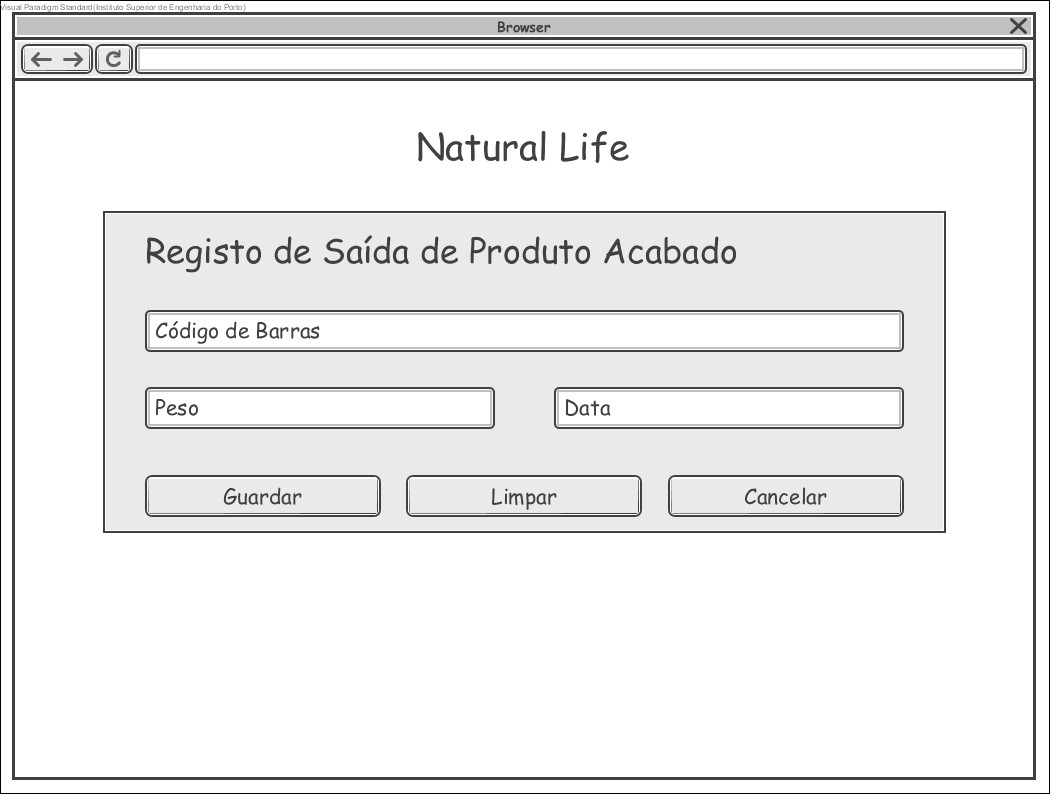
\includegraphics[width=\linewidth]{figuras/Diagramas_vp/DI_Fabrica_5_Saida_de_Produto_Acabado_1_Fase.jpg}
		\label{fig:di_saida_prod_acabado_1}
		\caption{Após concluir primeira fase}
	\end{subfigure}
	\begin{subfigure}[t]{0.45\linewidth}
		\includegraphics[width=\linewidth]{figuras/Diagramas_vp/DI_Fabrica_5_Saida_de_Produto_Acabado_2_Fase.jpg}
		\label{fig:di_saida_prod_acabado_2}
		\caption{Após concluir segunda fase}
	\end{subfigure}
	
	\caption{Modelo do menu}
	\label{fig:di_saida_prod_acabado}
\end{figure}

\subsubsection*{Fluxo do caso de utilização (2ª fase)}
O caso de uso inicia-se com a abertura da página do registo de saída de produto acabado. É apresentado o formulário com a data previamente preenchida. O utilizador tem de indicar o código de barras do produto acabado e o ID do cliente de uma lista \textit{dropdown}.  Após indicar as informações solicitadas precisona o botão "Guardar". No final do registo é apresentada uma mensagem ao utilizador. Caso o registo seja feito com sucesso um novo separador é aberto com o código de barras para ser impresso, tal como demonstrado na figura \ref{fig:sd_saida_prod_acabado}.


\begin{figure}[H] 
	\begin{center}
		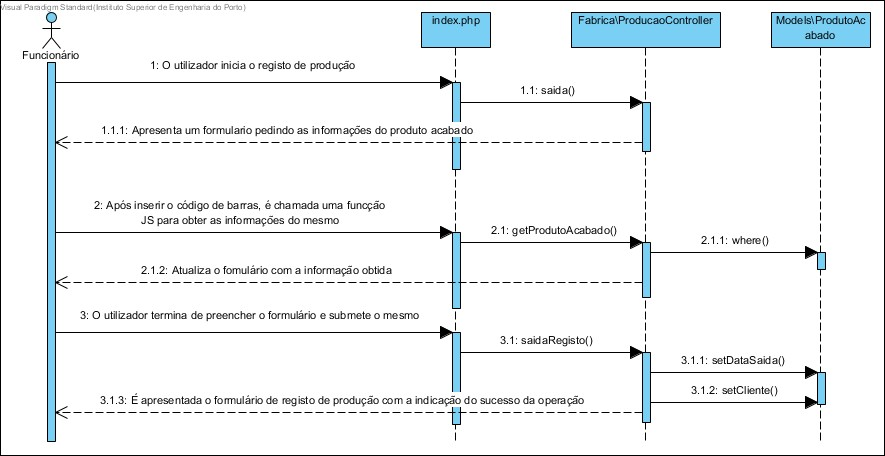
\includegraphics[width=0.95\textwidth,keepaspectratio]{figuras/Diagramas_vp/SD_Fabrica_5_Saida_de_Produto_Acabado.jpg}
		\caption{Diagrama de sequência registo de produto acabado}
		\label{fig:sd_saida_prod_acabado} 
	\end{center}
\end{figure}
\newpage
\subsection{Aplicação Fábrica: 2ª Via do código de barras}
\subsubsection*{Descrição do caso de uso}
Na obtenção de uma segunda via de um código de barras, espera-se que utilizador entre na página e indique o tipo de código de barras e o código de barras que pretende. 

\begin{figure}[H] 
	\begin{center}
		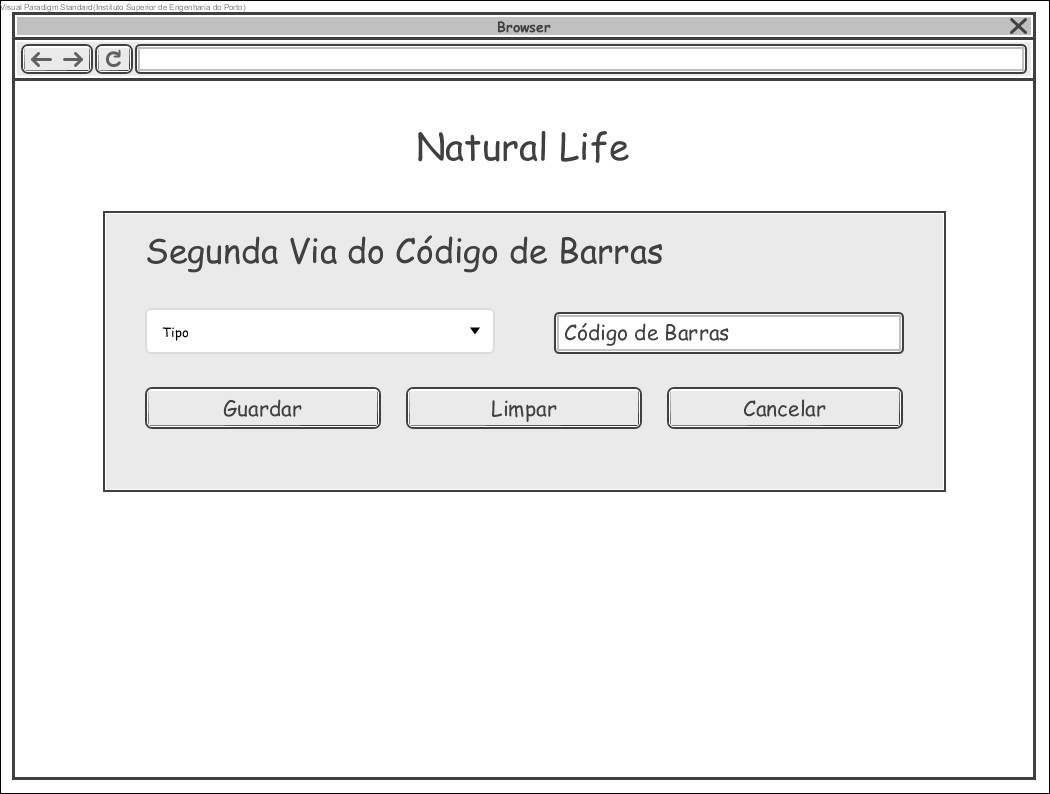
\includegraphics[width=0.60\textwidth,keepaspectratio]{figuras/Diagramas_vp/DI_Fabrica_6_2_Via_Codigo_de_Barras.jpg}
		\caption{Modelo do formulário de pedido de 2ª via de código de barras}
		\label{fig:di_2_via} 
	\end{center}
\end{figure}

\subsubsection*{Fluxo do caso de uso}
O caso de uso inicia-se com a abertura da página do pedido de segunda via de código de barras. É apresentado para o utilizador indicar o tipo de código de barras e o código de barras que pretende. Após indicar as informações solicitadas precisona o botão "Guardar". É aberto um novo separador com o código de barras solicitado para imprimir.

\todo{falta a image}
%\begin{figure}[H] 
%	\begin{center}
%		\includegraphics[width=\textwidth,keepaspectratio]{figuras/Diagramas_vp/SD_Fabrica_6_2_Via_Código_de_Barras.jpg}
%		\caption{Diagrama de sequência de pedido de 2ª via de código de barras}
%		\label{fig:sd_2_via} 
%	\end{center}
%\end{figure}
\newpage
\subsection{Aplicação Fábrica: Completar recolha}
\subsubsection*{Descrição do caso de uso}
Para completar recolha, espera-se que utilizador entre na página e indique o ID do ponto de recolha e o peso que pretende acrescentar à recolha. A informação sobre o peso total já registado bem como o histórico de incrementos será apresentado automaticamente pelo sistema. 

\begin{figure}[H] 
	\begin{center}
		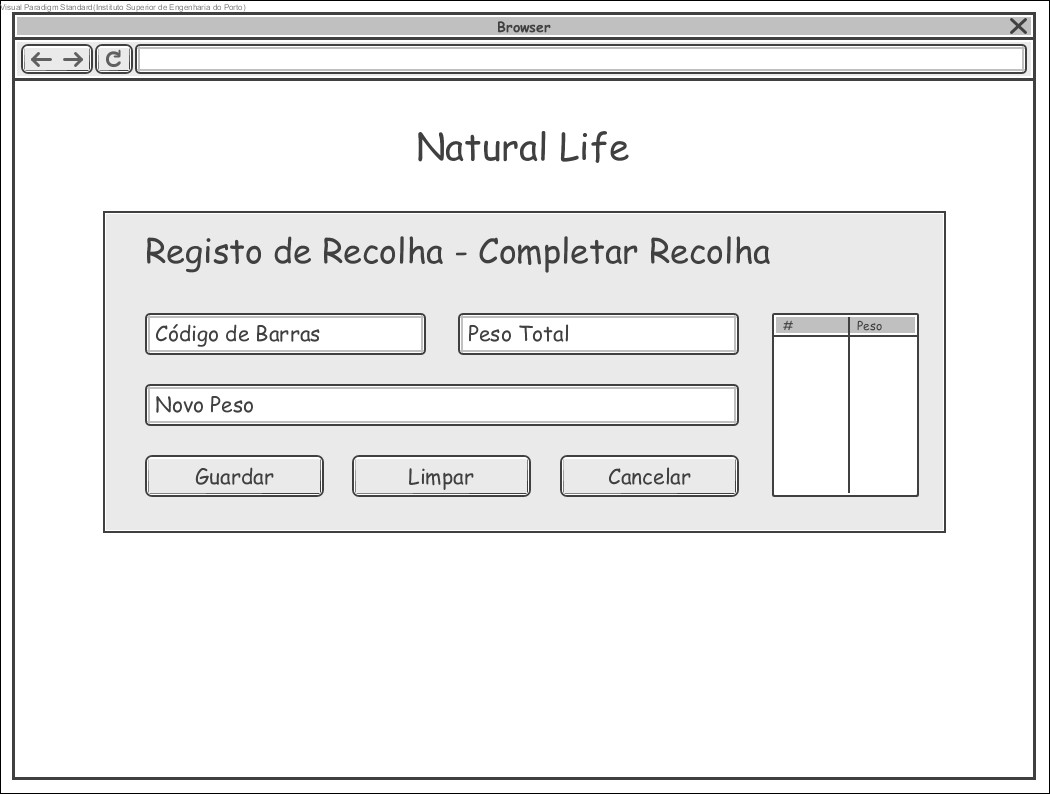
\includegraphics[width=0.60\textwidth,keepaspectratio]{figuras/Diagramas_vp/DI_Fabrica_7_Completa_Recolha.jpg}
		\caption{Modelo do formulário para incrementar o peso de uma recolha}
		\label{fig:di_completar_recolha} 
	\end{center}
\end{figure}

\subsubsection*{Fluxo do caso de uso}
O caso de uso inicia-se com a abertura da página do registo de recolha. É apresentado o formulário com a data previamente preenchida. O utilizador tem de indicar o ID do ponto de recolha numa lista de dropdown e o peso da recolha feita. Após indicar as informações solicitadas precisona o botão "Guardar". No final do registo é apresentada uma mensagem ao utilizador. Caso o registo seja feito com sucesso um novo separador é aberto com o código de barras para ser impresso.


\begin{figure}[h!] 
	\begin{center}
		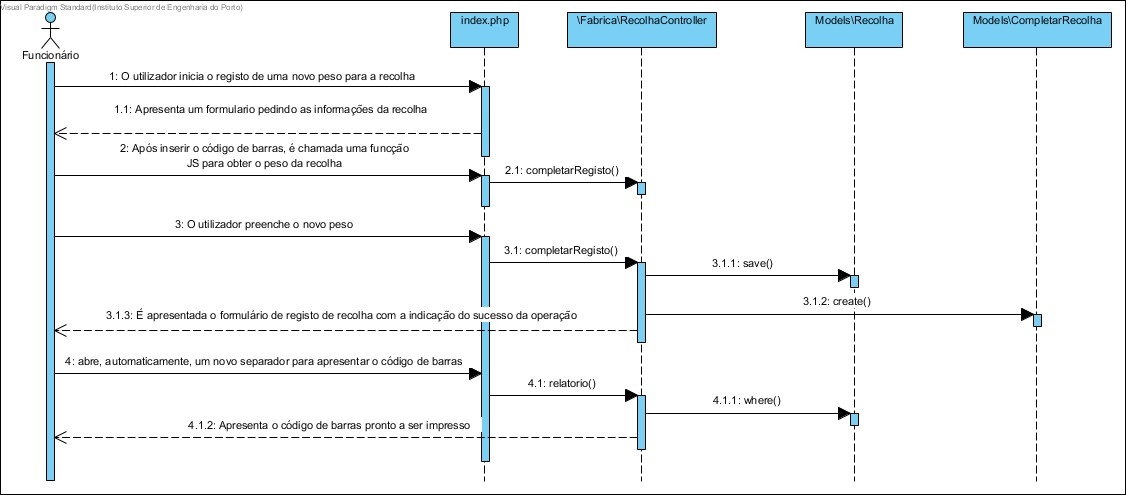
\includegraphics[width=0.90\textwidth,keepaspectratio]{figuras/Diagramas_vp/SD_Fabrica_7_Completar_Recolha.jpg}
		\caption{Diagrama de sequência para incrementar o peso de uma recolha}
		\label{fig:sd_completar_recolha} 
	\end{center}
\end{figure}
\newpage

% Aplicação Painel
\subsection{Aplicação Painel - Nota introdutória}
Os casos de uso na aplicação painel são todos iguais, independentemente do model. Desde que o caso de uso se enquadre num determinado model, os esquemas apresentados são válidos para esse model. Por esse motivo optou-se por apresentar apenas um tópico para cada caso de uso e nele é indicado os models que são compatíveis.

\subsection{Aplicação Painel - Listagem}
\subsubsection*{Descrição do caso de uso}
Para fazer uma listagem, utilizador apenas necessita de entrar na página. A aparência da \textit{view} deste caso de utilização será semelhante ao demonstrado na figura \ref{fig:di_lista}. 

\begin{figure}[H] 
	\begin{center}
		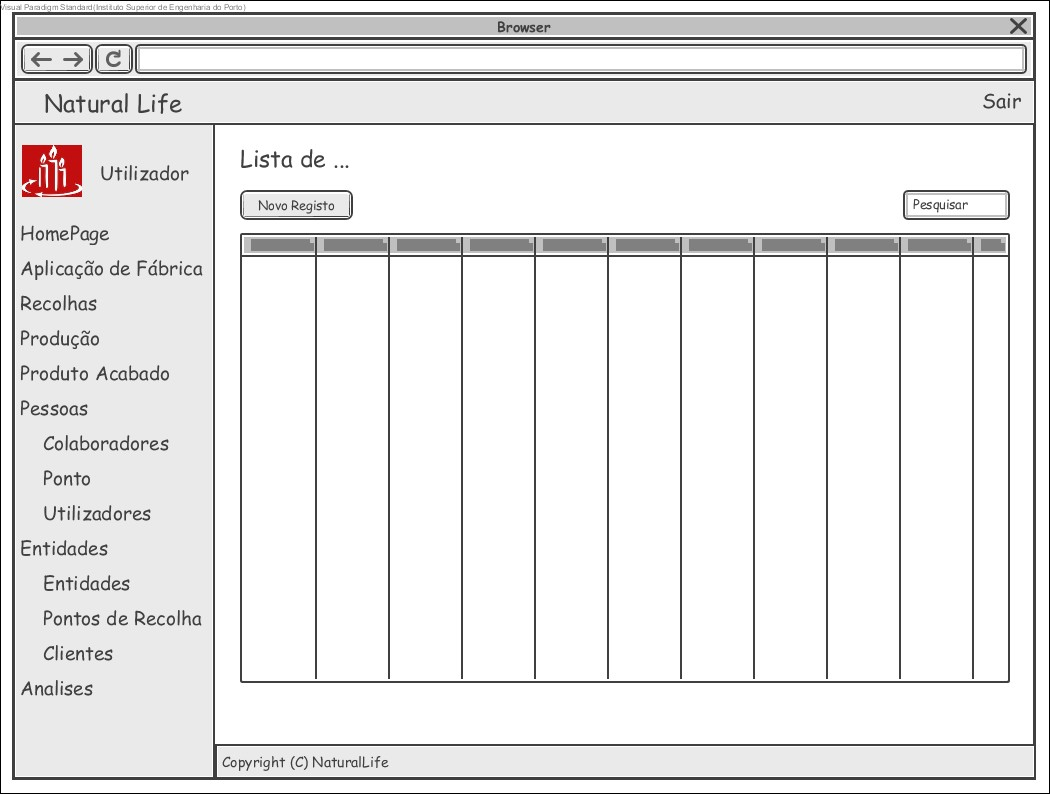
\includegraphics[width=0.60\textwidth,keepaspectratio]{figuras/Diagramas_vp/DI_Painel_1_Lista.jpg}
		\caption{Modelo da página de listagem}
		\label{fig:di_lista} 
	\end{center}
\end{figure}

\subsubsection*{Models compatíveis com o caso de uso}
Todos os models são compatíveis com este caso de uso

\subsubsection*{Fluxo do caso de utilização}
O caso de uso inicia-se com a abertura da página de listagem. É apresentado uma tabela com os dados listado e algumas opções para cada linha, tal como demonstrado na figura \ref{fig:sd_lista}.


\begin{figure}[H] 
	\begin{center}
		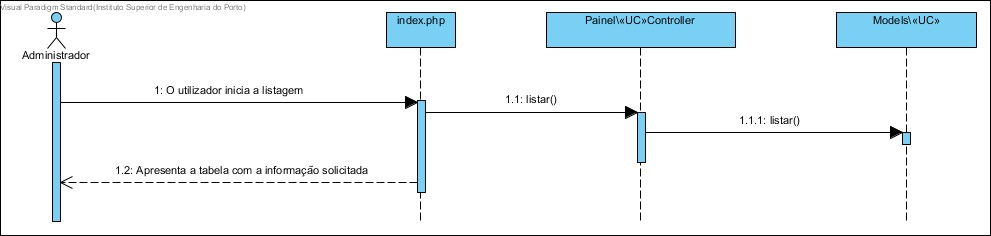
\includegraphics[width=\textwidth,keepaspectratio]{figuras/Diagramas_vp/SD_Painel_1_Listar.jpg}
		\caption{Diagrama de sequência da listagem}
		\label{fig:sd_lista} 
	\end{center}
\end{figure}
\newpage
\subsection{Aplicação Painel - Inserir}
\subsubsection*{Descrição do caso de uso}
Para inserir um registo, o utilizador necessita pressionar o botão \textit{Novo Registo}. A aparência da \textit{view} deste caso de utilização será semelhante ao demonstrado na figura \ref{fig:di_novo}. 

\begin{figure}[H] 
	\begin{center}
		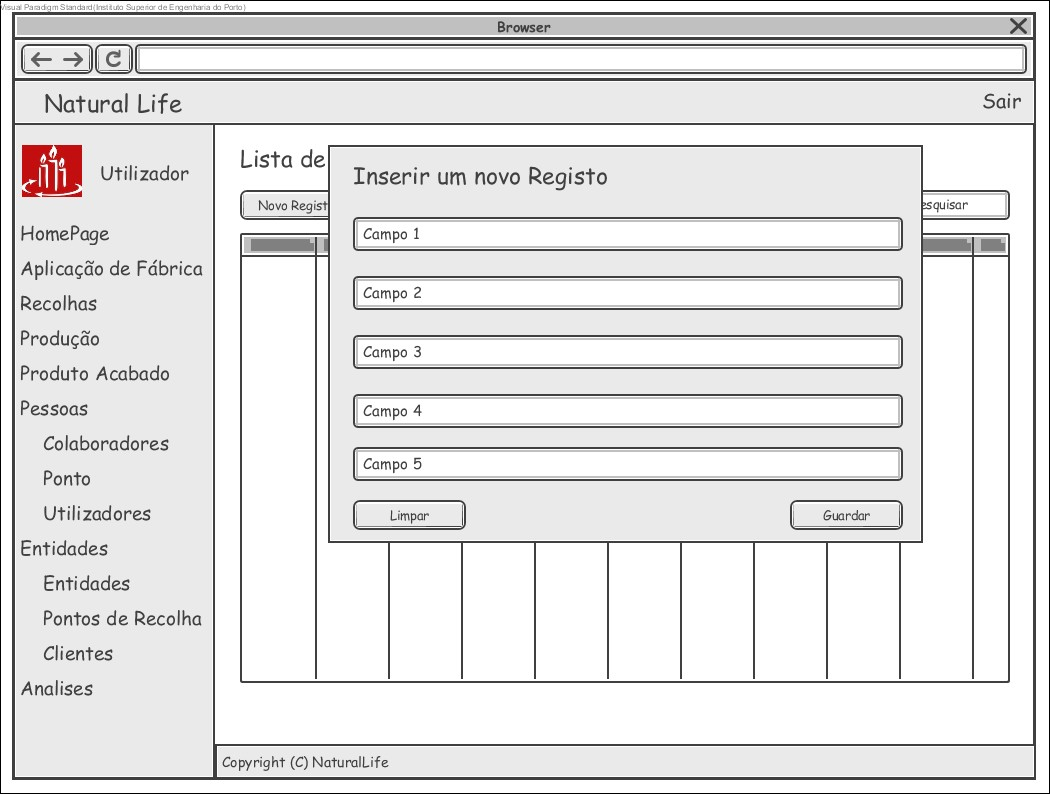
\includegraphics[width=0.60\textwidth,keepaspectratio]{figuras/Diagramas_vp/DI_Painel_2_Inserir.jpg}
		\caption{Modelo da janela de inserção na página de listagem}
		\label{fig:di_novo} 
	\end{center}
\end{figure}

\subsubsection*{\textit{Models} compatíveis com o caso de uso}
Todos os \textit{models} são compatíveis com este caso de uso

\subsubsection*{Fluxo do caso de utilização}
O caso de uso inicia-se quando o utilizador pressionar o botão novo registo na página de listagem. É apresentado uma janela flutuante com com os campos a serem preenchidos. O utilizador preenche os campos e pressiona o botão guardar. Finalizado o registo a janela fecha-se e é apresentado uma mensagem ao utilizador, tal como demonstrado na figura \ref{fig:sd_novo}.


\begin{figure}[H] 
	\begin{center}
		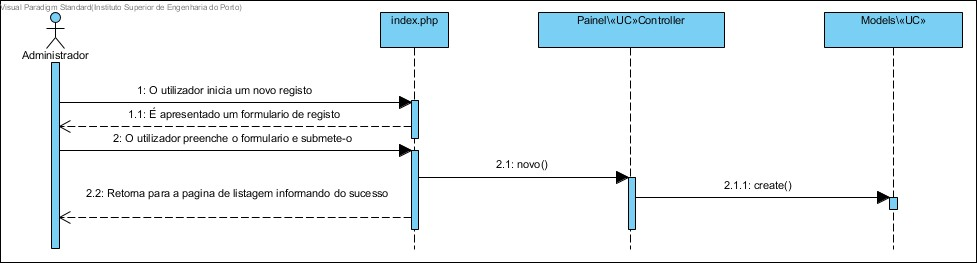
\includegraphics[width=\textwidth,keepaspectratio]{figuras/Diagramas_vp/SD_Painel_2_Inserir.jpg}
		\caption{Diagrama de sequência de inserir registo}
		\label{fig:sd_novo} 
	\end{center}
\end{figure}
\newpage
\subsection{Aplicação Painel - Editar}
\subsubsection*{Descrição do caso de uso}
Para editar um registo, o utilizador necessita pressionar o botão \textit{editar} na linha referente ao registo que pretende atualizar. A aparência da \textit{view} deste caso de utilização será semelhante ao demonstrado na figura \ref{fig:di_editar}. 

\begin{figure}[H] 
	\begin{center}
		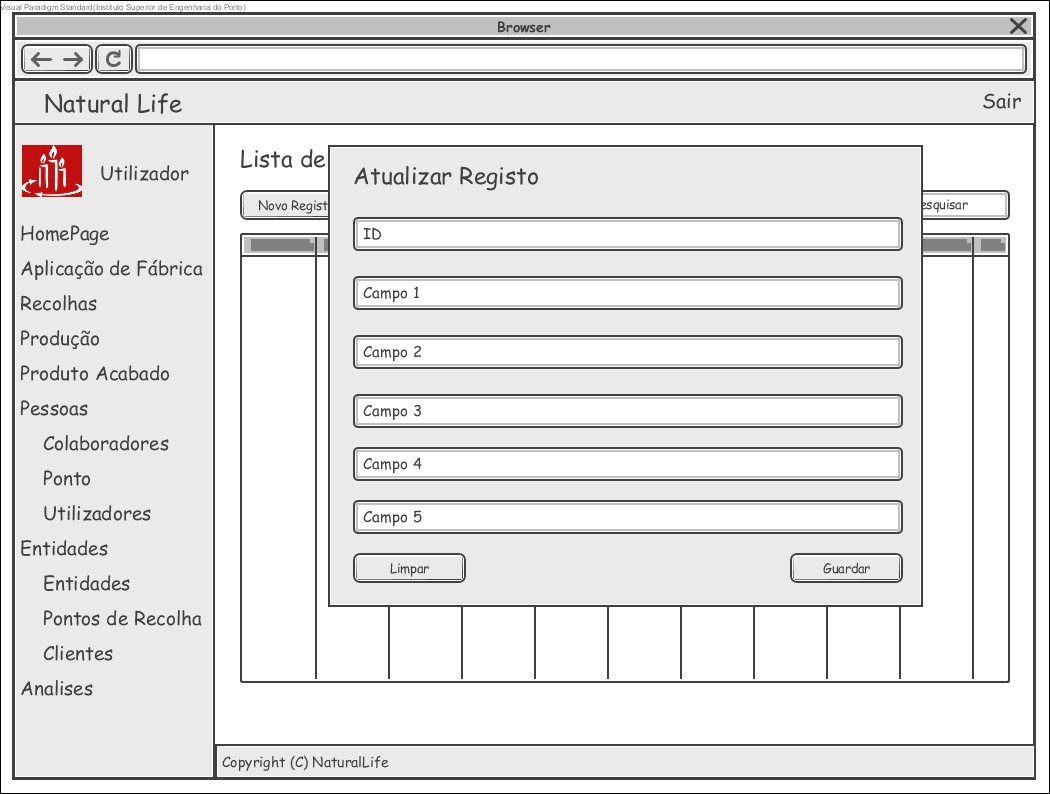
\includegraphics[width=0.60\textwidth,keepaspectratio]{figuras/Diagramas_vp/DI_Painel_3_Editar.jpg}
		\caption{Modelo da janela de edição na página de listagem}
		\label{fig:di_editar} 
	\end{center}
\end{figure}

\subsubsection*{\textit{Models} compatíveis com o caso de uso}
Este caso de uso é compatível com os \textit{models} Recolha, Produção, Produto Acabado, Colaboradores, Registo de Ponto, Entidades, Pontos de Recolha, Clientes e Analises.

\subsubsection*{Fluxo do caso de utilização}
O caso de uso inicia-se quando o utilizador pressionar o botão editar da linha do registo que pretende atualizar. O sistema vai fazer um request em background para obter as informações da base de dados e apresenta uma janela flutuante com com os campos a serem pré-preenchidos com as informações recebidas. O utilizador faz as alterações que pretende e pressiona o botão guardar. Finalizado o registo a janela fecha-se e é apresentado uma mensagem ao utilizador.


\begin{figure}[H] 
	\begin{center}
		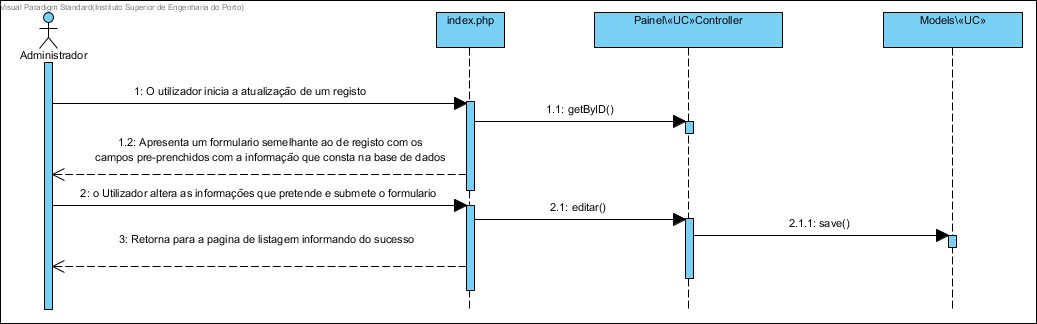
\includegraphics[width=\textwidth,keepaspectratio]{figuras/Diagramas_vp/SD_Painel_3_Editar.jpg}
		\caption{Diagrama de sequência de editar registo}
		\label{fig:sd_editar} 
	\end{center}
\end{figure}
\newpage
\subsection{Aplicação Painel: Apagar}
\subsubsection*{Descrição do caso de uso}
Para apagar um registo, o utilizador necessita pressionar o botão \textit{apagar} na linha referente ao registo que pretende atualizar. Pelo facto de ser apenas uma procedimento executado em \textit{background}, não possui nenhuma \textit{view}.

\subsubsection*{\textit{Models} compatíveis com o caso de uso}
Este caso de uso é compatível com os \textit{models} Recolha, Produção, Produto Acabado, Colaboradores, Registo de Ponto, Utilizadores, Pontos de Recolha, Clientes e Analises.

\subsubsection*{Fluxo do caso de utilização}
O caso de uso inicia-se quando o utilizador pressionar o botão apagar da linha do registo que pretende \textit{apagar}. É apresentada uma janela de confirmação. Após executar a ação é apresentada uma mensagem ao utilizador, tal como demonstrado na figura \ref{fig:sd_apagar}


\begin{figure}[H] 
	\begin{center}
		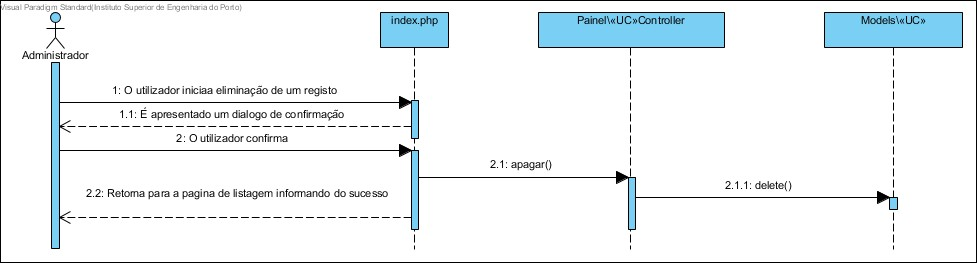
\includegraphics[width=\textwidth,keepaspectratio]{figuras/Diagramas_vp/SD_Painel_4_Apagar.jpg}
		\caption{Diagrama de sequência de apagar registo}
		\label{fig:sd_apagar} 
	\end{center}
\end{figure}
\newpage
\subsection{Aplicação Painel: Desativar/Ativar}
\subsubsection*{Descrição do caso de uso}
Desativar um registo significa que este se vai manter na base de dados, mas não irá constar mais nas UI da aplicação de Fábrica. Para \textit{desativar/ativar} um registo, o utilizador necessita pressionar o botão \textit{desativar/ativar} na linha referente ao registo que pretende atualizar. Pelo facto de ser apenas uma procedimento executado em \textit{background}, não possui nenhuma view.

\subsubsection*{\textit{Models} compatíveis com o caso de uso}
Este caso de uso é compatível com os \textit{models} Colaboradores, Pontos de Recolha e Clientes.

\subsubsection*{Fluxo do caso de utilização}
O caso de uso inicia-se quando o utilizador pressionar o botão desativar/ativar da linha do registo que pretende desativar/ativar. Após executar a ação é apresentada uma mensagem ao utilizador, tal como demonstrado na figura \ref{fig:sd_desativar}


\begin{figure}[H] 
	\begin{center}
		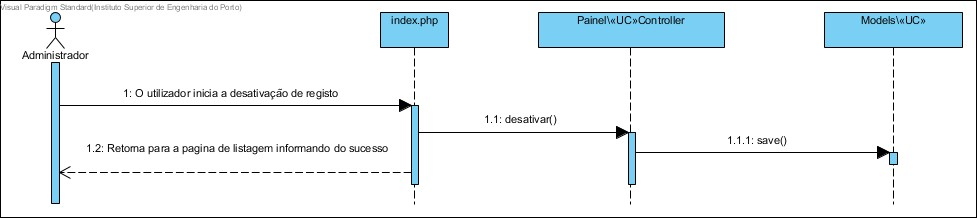
\includegraphics[width=\textwidth,keepaspectratio]{figuras/Diagramas_vp/SD_Painel_5_Desativar.jpg}
		\caption{Diagrama de sequência de desativar/ativar registo}
		\label{fig:sd_desativar} 
	\end{center}
\end{figure}
\newpage
\subsection{Aplicação Painel - segunda via código de barras}
\subsubsection*{Descrição do caso de uso}
Caso pretenda, um utilizador do painel também pode re-imprimir um código de barras sem necessidade de abrir a aplicação Fábrica. Para isso o utilizador necessita pressionar o botão\textit{ segunda via} da linha referente ao registo que pretende atualizar. Pelo facto de ser apenas uma procedimento executado em \textit{background}, não possui nenhuma \textit{view}.

\subsubsection*{\textit{Models} compatíveis com o caso de uso}
Este caso de uso é compatível com os \textit{models} Recolhas, Produto Acabado.

\subsubsection*{Fluxo do caso de utilização}
O caso de uso inicia-se quando o utilizador pressionar o botão 2ª via de código de barras da linha do registo. Um novo separador abre-se com o código de barras pronto a ser impresso, tal como demonstrado na figura \ref{fig:sd_2_via_painel}.


\begin{figure}[H] 
	\begin{center}
		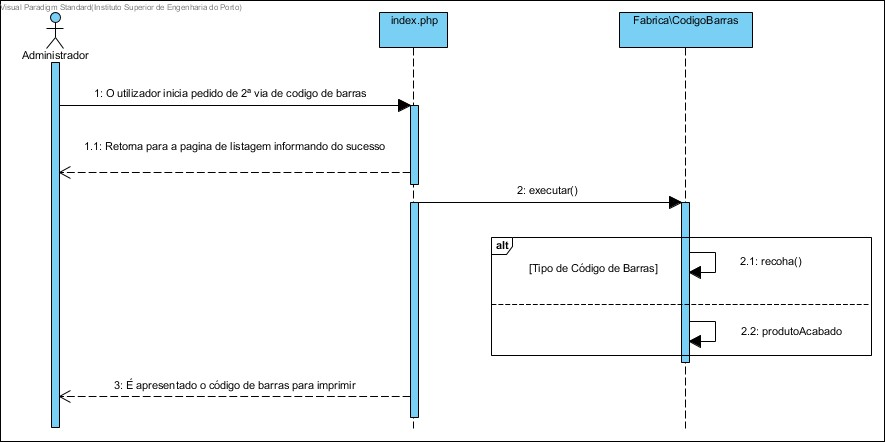
\includegraphics[width=\textwidth,keepaspectratio]{figuras/Diagramas_vp/SD_Painel_6_2_via_Codigo_de_Barras.jpg}
		\caption{Diagrama de sequência imprimir 2ª via do código de barras}
		\label{fig:sd_2_via_painel} 
	\end{center}
\end{figure}
\cleardoublepage
% ************ Chapter 5 ************
\chapter{Título Capítulo 5} 
\label{cap:5}
\emph{Breve introdução ao Capítulo 5.}


\section{Primeira secção do Capítulo 5}

....

\subsection{Primeira subsecção do Capítulo 5}

....





\section{Conclusão do Capítulo 5}

Breve conclusão do Capítulo 5.
\cleardoublepage
% ************ Chapter 7 ************
\chapter{Conclusões}
\label{cap:6}
O capítulo de conclusões é um dos mais importantes do relatório, sendo aqui que devem ser apresentados os resultados do trabalho efetivamente desenvolvido. 
As conclusões finais devem focar o sucesso/insucesso do trabalho, revendo as dificuldades encontradas. Devem resumir, de alguma forma, as vantagens do produto desenvolvido e a utilidade que possa ter para a instituição de estágio ou para os seus clientes/parceiros. Podem também referir a forma como o estágio decorreu, bem como a integração, a formação dada pela instituição, as facilidades e as dificuldades sentidas ao longo do estágio.
As conclusões devem basear-se nos resultados realmente obtidos. Devem enquadrar-se os resultados obtidos com os objetivos enunciados e procurar extrair conclusões mais gerais, eventualmente sugeridas pelos resultados. Podem acompanhar as conclusões incluindo recomendações apropriadas, resultantes do trabalho, nomeadamente sugerindo e justificando eventuais extensões e modificações futuras.


\section{Resumo do relatório}

Esta secção é opcional, servindo apenas para relembrar os pontos mais importantes focados nos capítulos anteriores.


\section{Objetivos realizados}

Nesta secção devem ser repetidos os objetivos apresentados no capítulo de introdução e, para cada um deles, deve ser descrito o seu grau de realização. Recomenda-se o uso de uma lista, dado que facilita a compreensão pelo leitor.

\section{Limitações e trabalho futuro}

Nesta secção devem ser identificados os limites do trabalho realizado (condições de operação), fazendo uma análise autocrítica ao trabalho, bem como extrapolar sobre as possíveis direções de desenvolvimento futuro.

\section{Apreciação final}

Esta secção deve fornecer uma opinião pessoal sobre o trabalho desenvolvido. Nomeadamente o seu contributo para o desenvolvimento pessoal e profissional.
\cleardoublepage
% *************** Bibliografia *********************
\renewcommand*\bibname{Referências Bibliográficas}
\bibliographystyle{ieeetr}
\bibliography{bibliografia}
\cleardoublepage
% *************** Anexos ***************************
\renewcommand{\appendixname}{Anexo}
\appendix
% ************ Anexo  ************
\renewcommand{\appendixname}{Anexo}
\appendix
\chapter{Documento com as alternativas para o desenvolvimento do projeto entregue à administração}
\label{anexo:A}

O documento a seguir foi produzido para informar a administração das diferentes opções tecnológicas para o desenvolvimento da plataforma solicitada pela empresa.

\newpage

\begin{figure}[H]
	\centering
	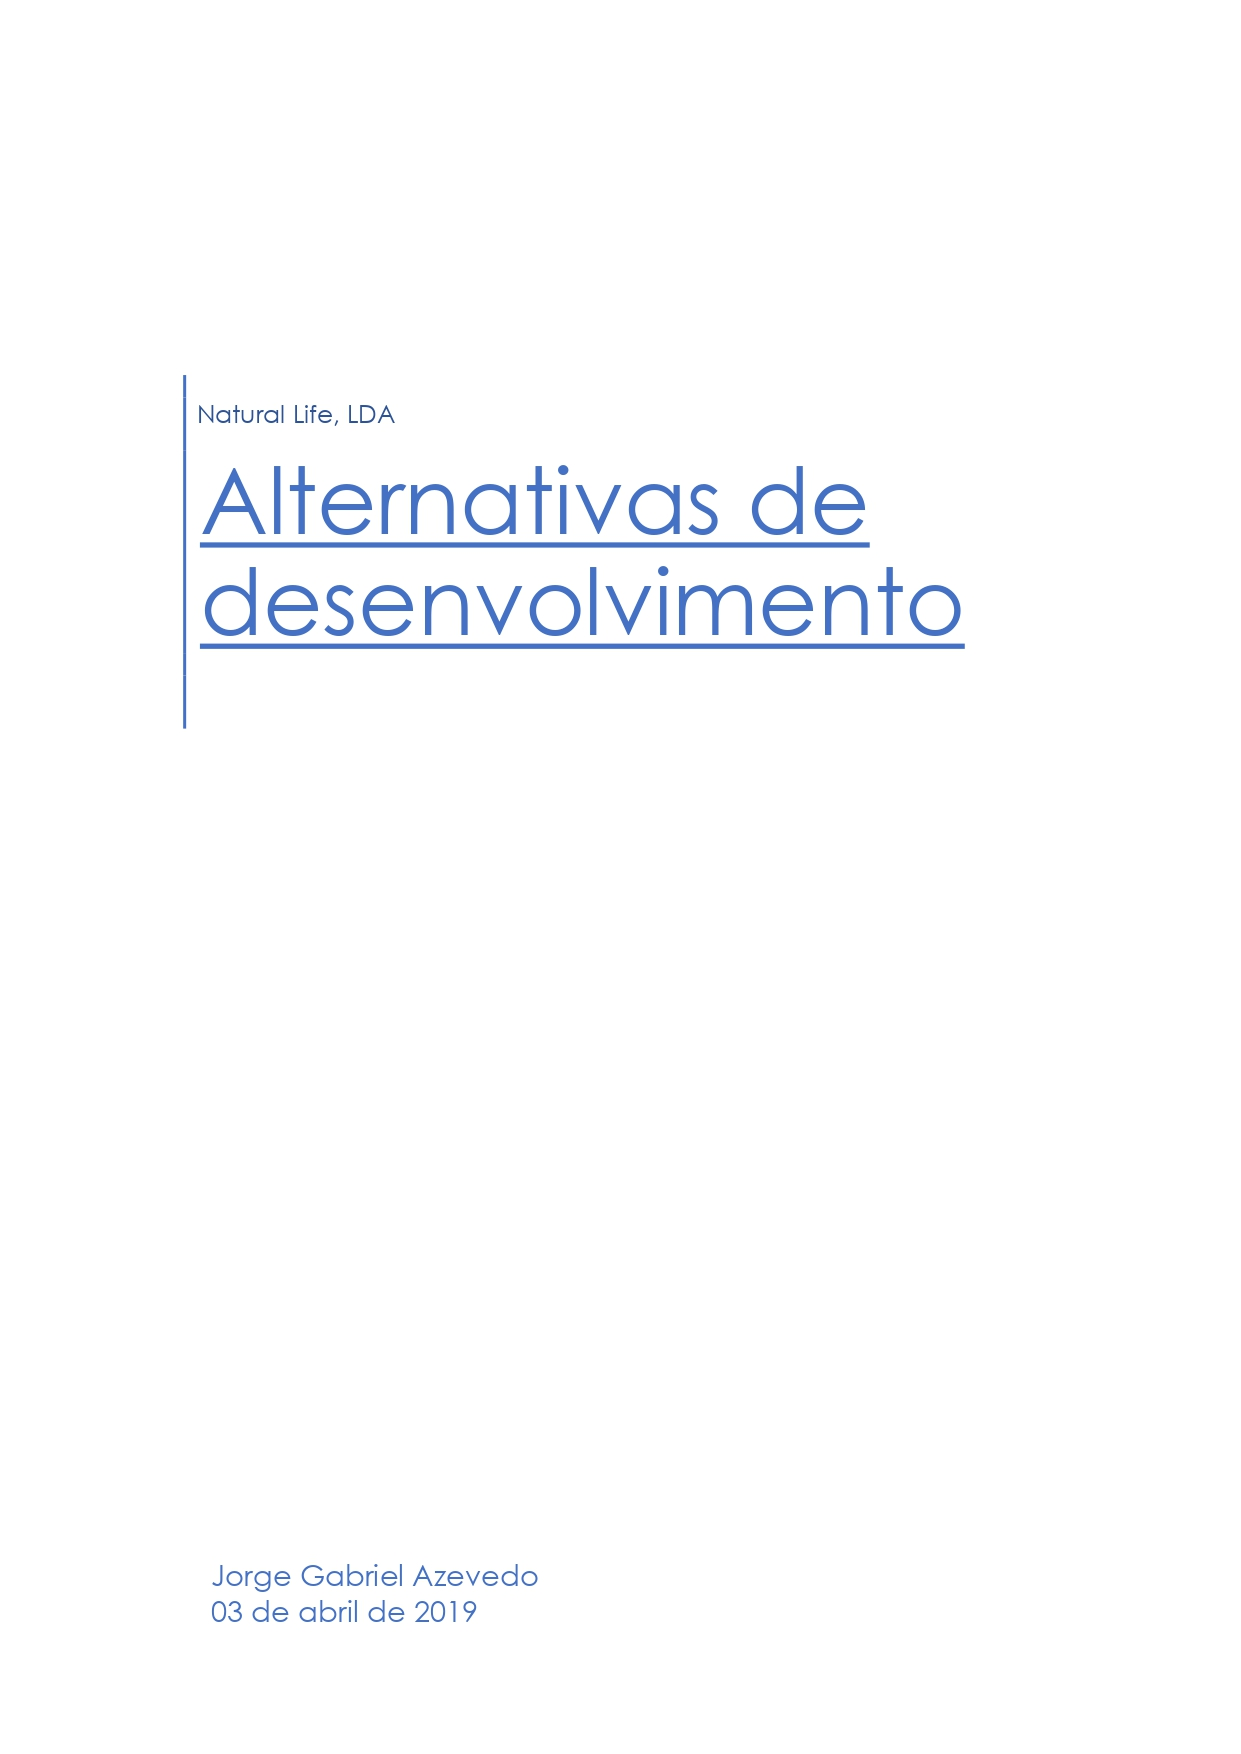
\includegraphics[width=\linewidth, frame]{figuras/Alternativas/pag0.jpg}
	\caption{Capa do documento}
	\label{fig:anexo_a_capa}
\end{figure}
\newpage

\begin{figure}[H]
	\centering
	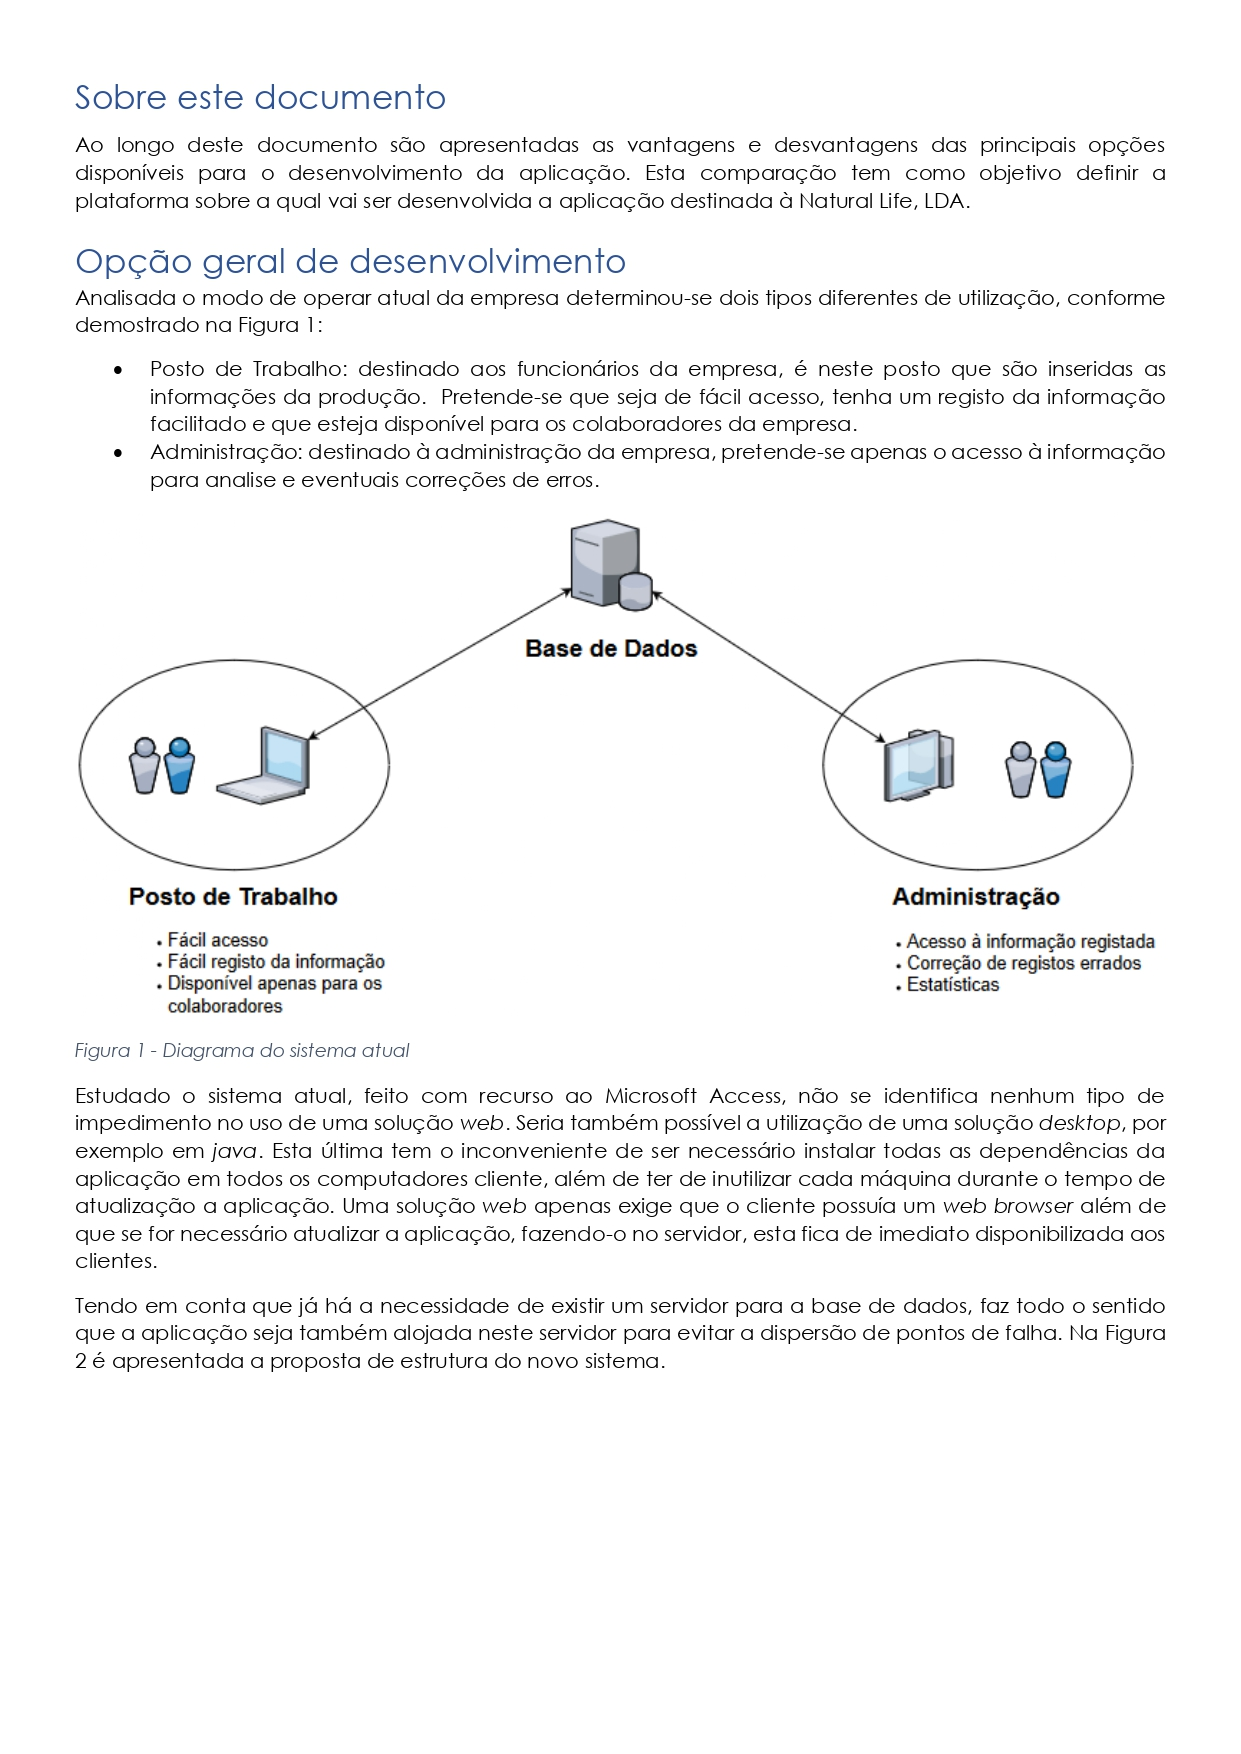
\includegraphics[width=\linewidth, frame]{figuras/Alternativas/pag1.jpg}
	\caption{Página 1}
	\label{fig:anexo_a_1}
\end{figure}
\newpage

\begin{figure}[H]
	\centering
	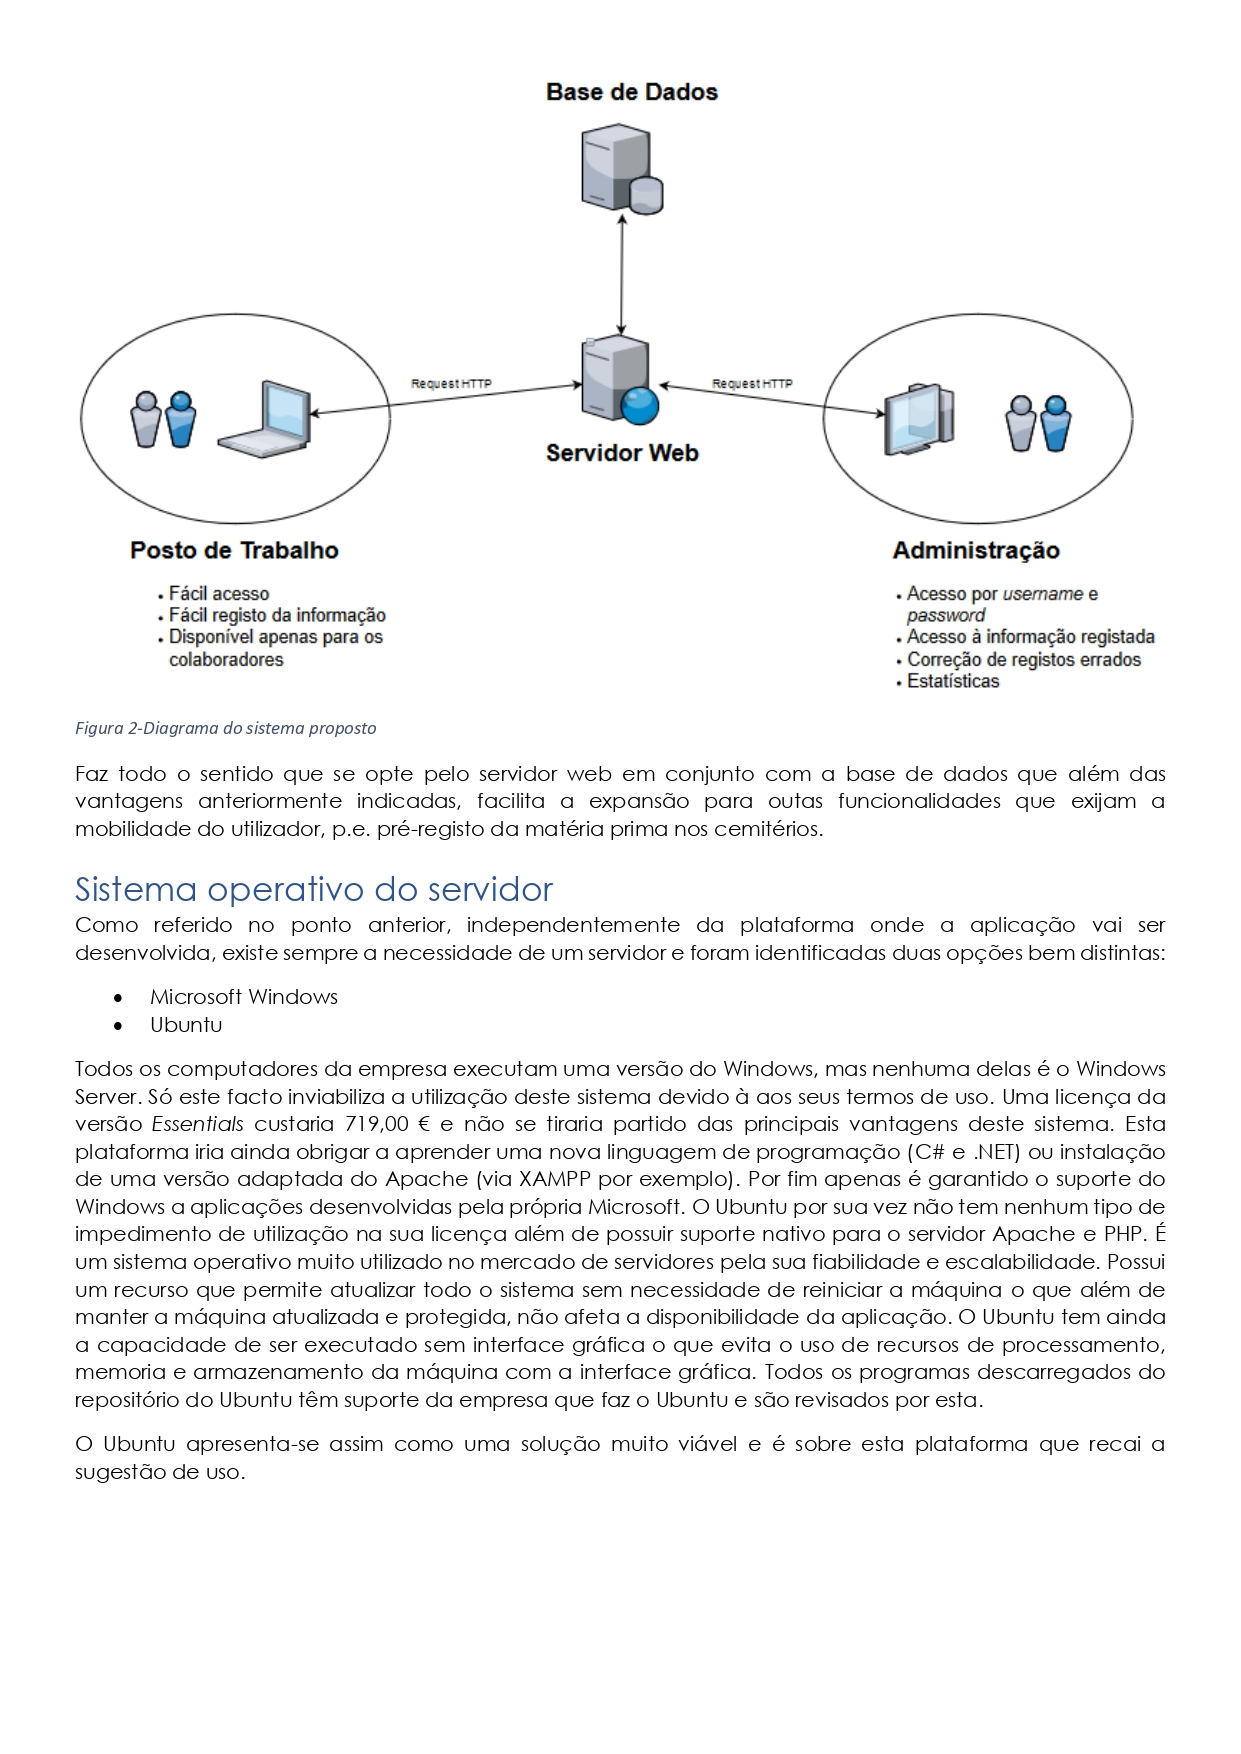
\includegraphics[width=\linewidth, frame]{figuras/Alternativas/pag2.jpg}
	\caption{Página 2}
	\label{fig:anexo_a_2}
\end{figure}
\newpage

\begin{figure}[H]
	\centering
	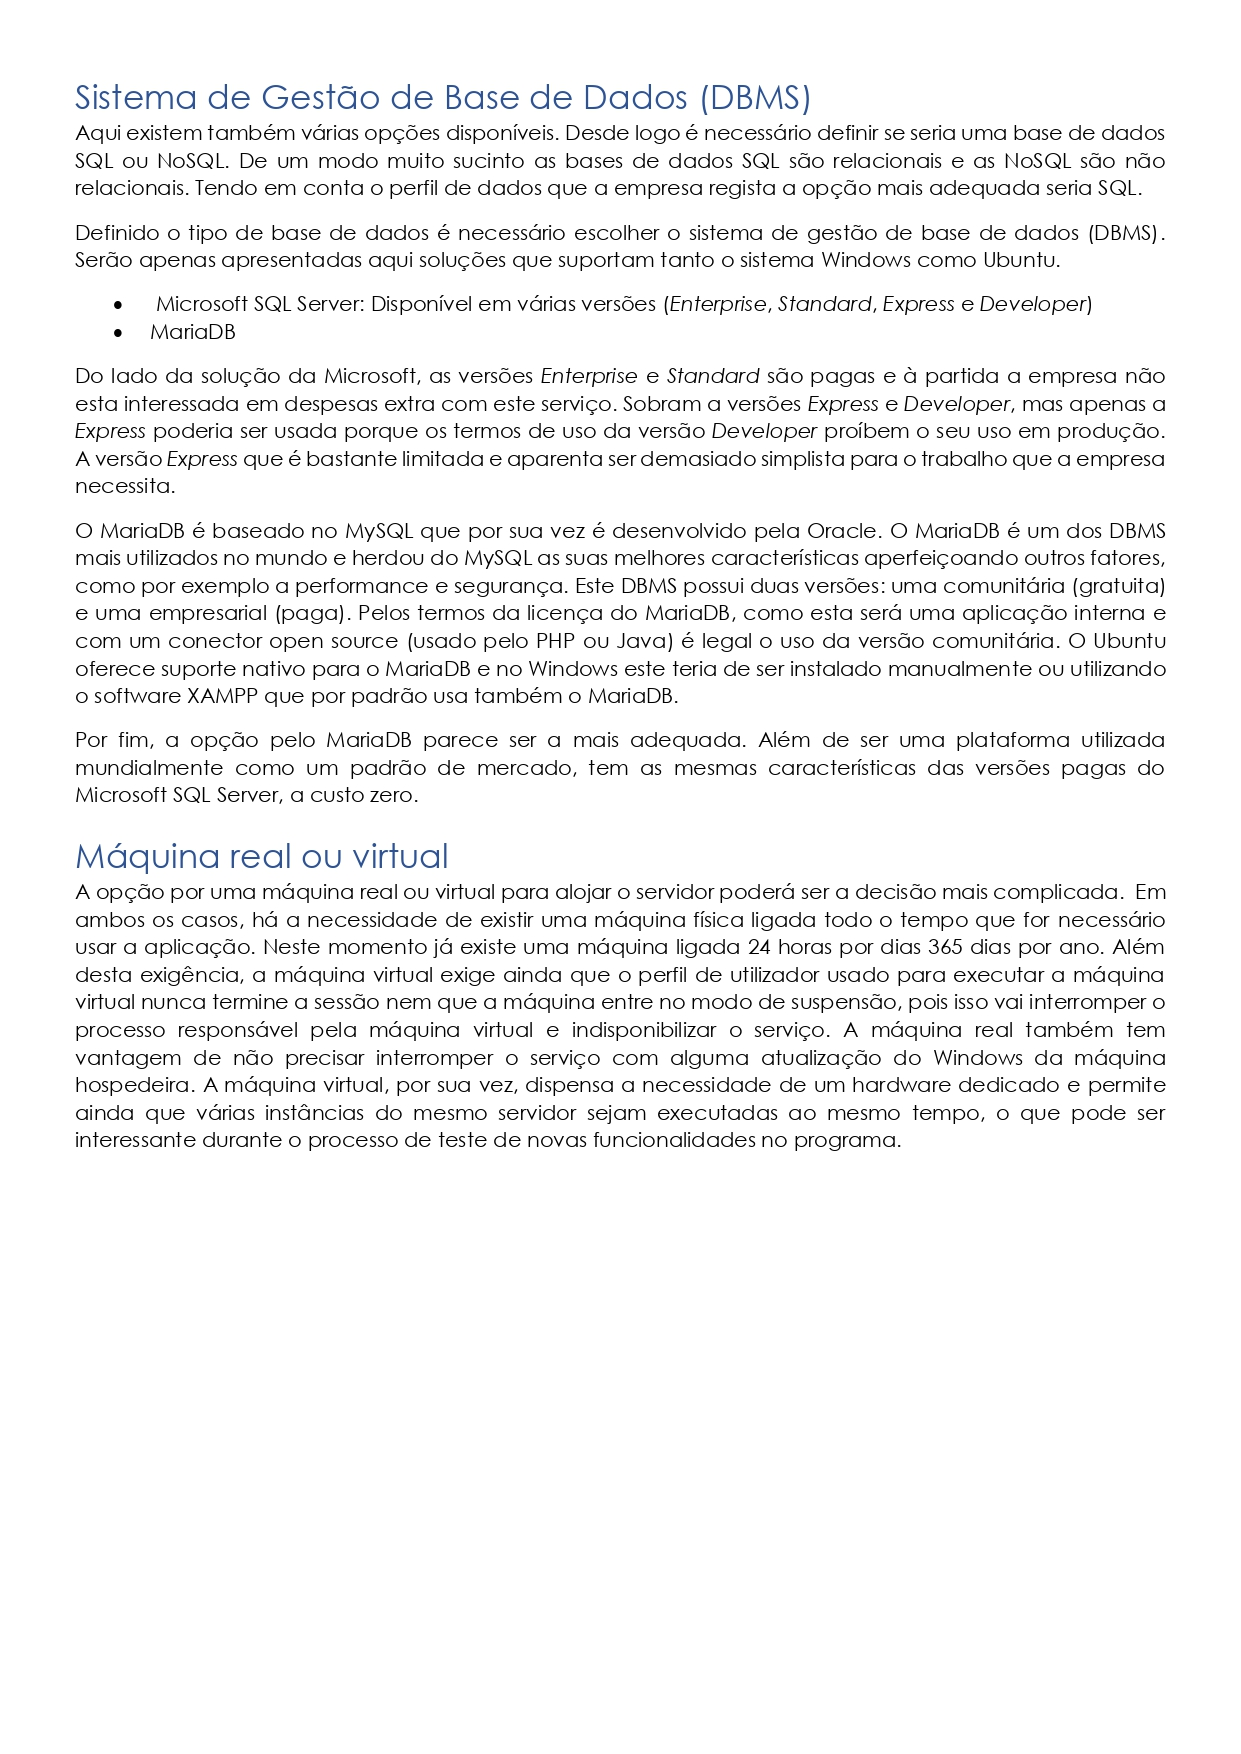
\includegraphics[width=\linewidth, frame]{figuras/Alternativas/pag3.jpg}
	\caption{Página 3}
	\label{fig:anexo_a_3}
\end{figure}
\newpage

\begin{figure}[H]
	\centering
	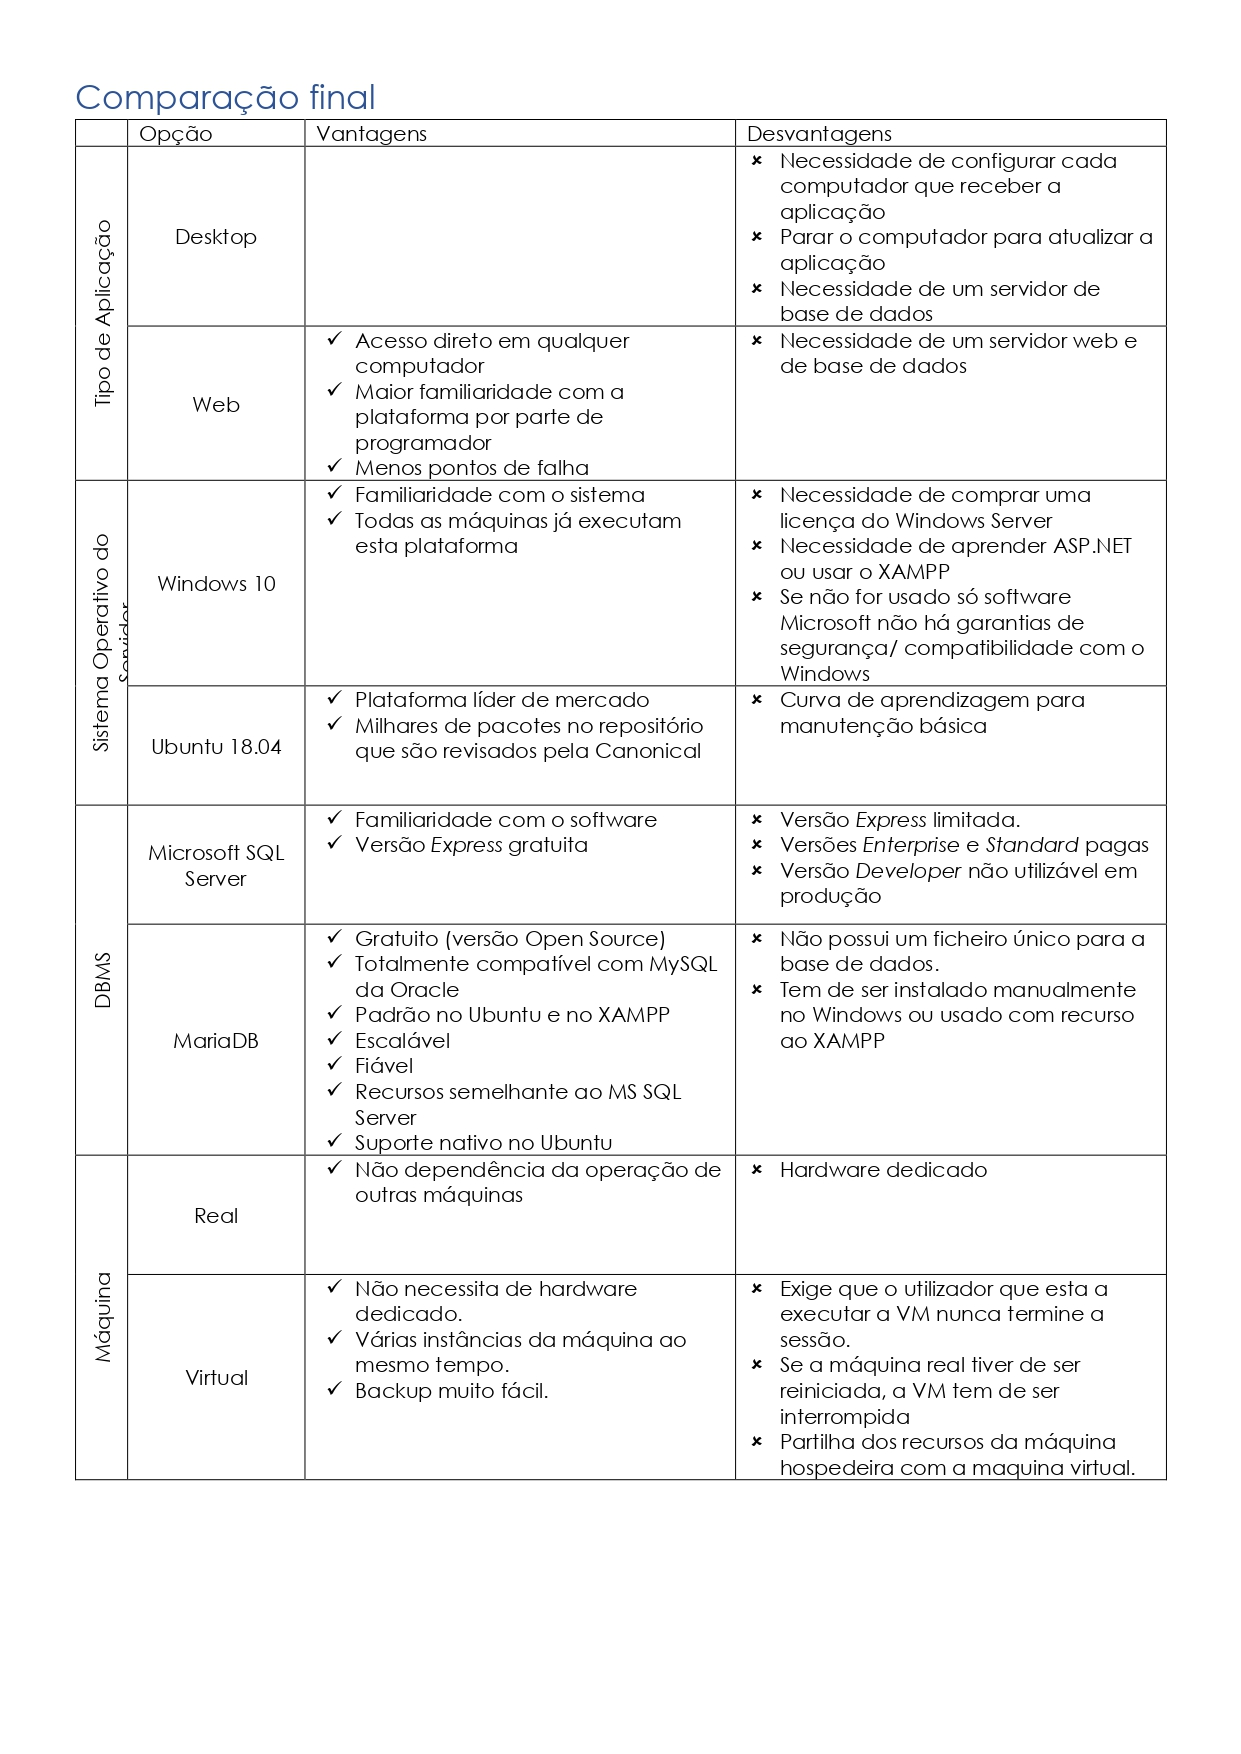
\includegraphics[width=\linewidth, frame]{figuras/Alternativas/pag4.jpg}
	\caption{Página 4}
	\label{fig:anexo_a_4}
\end{figure}
\newpage

\begin{figure}[H]
	\centering
	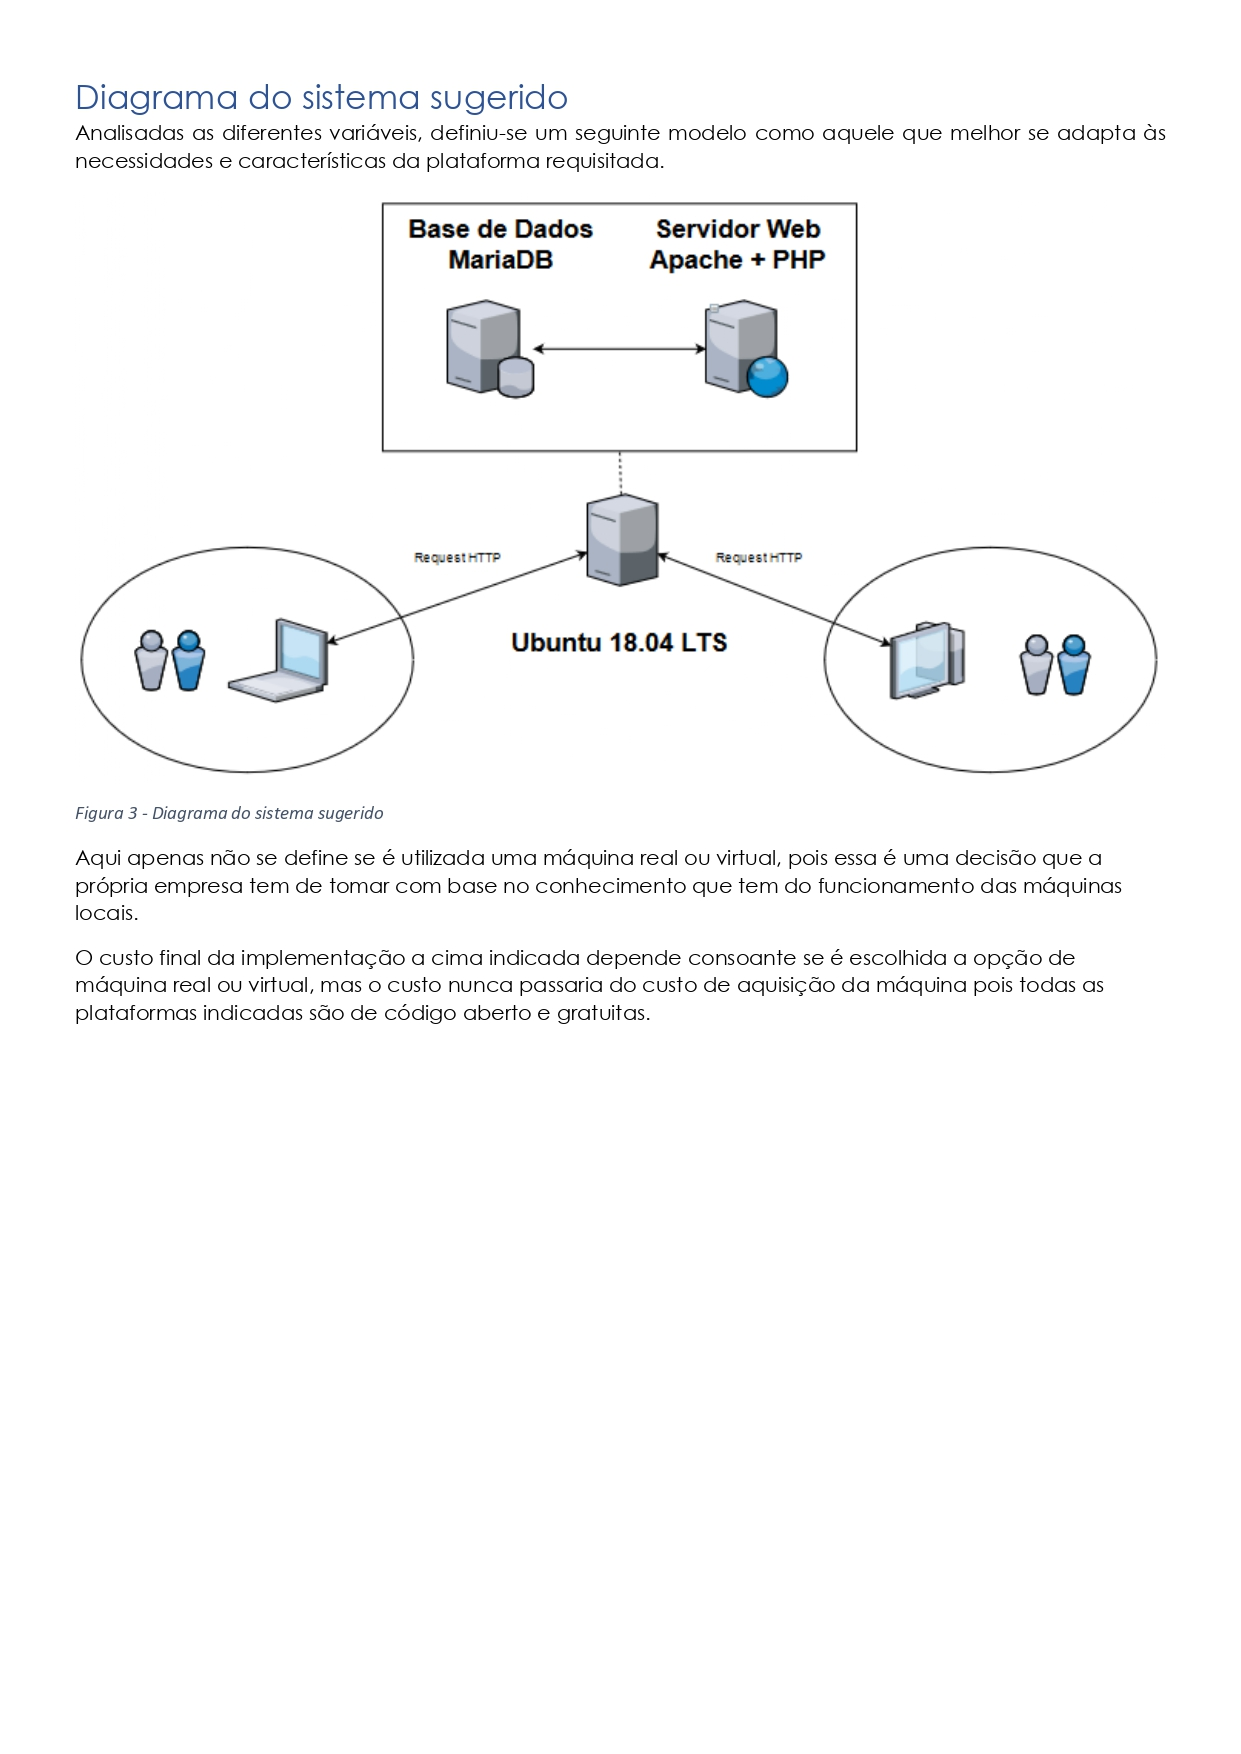
\includegraphics[width=\linewidth, frame]{figuras/Alternativas/pag5.jpg}
	\caption{Página 5}
	\label{fig:anexo_a_5}
\end{figure}
\cleardoublepage
%% ************ Anexo  ************
%\renewcommand{\appendixname}{Anexo}
%\appendix % Usar este comando só no primeiro Anexo
\chapter{Título do Anexo B}
\label{anexo:B}

....


%\cleardoublepage
%% ************ Anexo  ************
%\renewcommand{\appendixname}{Anexo}
%\appendix % Usar este comando só no primeiro Anexo
\chapter{\textit{Stored procedure} fim de protocolo}
\label{anexo:C}
Código utilizado na \textit{stored procedure Fim de Protocolo} para notificar a administração da empresa sobre quais Pontos de Recolha cujo o protocolo está prestes terminar.

\begin{verbatim}
USE [NaturalLife]
GO
/****** Object:  StoredProcedure [dbo].[FimProtocolos]    
Script Date: 16/07/2019 08:38:38 ******/
SET ANSI_NULLS ON
GO
SET QUOTED_IDENTIFIER ON
GO
-- =============================================
-- Author:		NaturalLife
-- Create date: 03-07-2019
-- Description:	Alerta pontos de recolha
-- =============================================
ALTER PROCEDURE [dbo].[FimProtocolos]
AS
BEGIN

--params 1º alerta: 90 dias, 2º alerta: 30 dias, 3º alerta: 15 dias
DECLARE @Alerta1 AS INT = 90 -- 1º Alerta
DECLARE @Alerta2 AS INT = 30 -- 2º Alerta
--DECLARE @Alerta3 AS INT = 0 -- 3º Alerta


IF EXISTS(SELECT
pontos_recolha.id,
pontos_recolha.nome,
pontos_recolha.fimProtocolo,
DATEDIFF(day, GETDATE(), pontos_recolha.fimProtocolo)
FROM pontos_recolha
WHERE   
DATEDIFF(day, GETDATE(), pontos_recolha.fimProtocolo) 
in (@Alerta1, @Alerta2))
BEGIN

--Declara as variaveis
Declare @HTMLBody nvarchar(max),
@tableBody nvarchar(max)

--Cria a tabela HTML
SET @tableBody = CONVERT(NVARCHAR(MAX), (SELECT
(SELECT '' FOR XML PATH(''), TYPE) AS 'caption',
(SELECT 
'ID' AS th,
'Nome' AS th,
'Fim do protocolo' AS th,
'Dias Restantes' AS th 
FOR XML RAW('tr'), ELEMENTS, TYPE) AS 'thead',
(

--Inicio da Query
SELECT
pontos_recolha.id as td,
pontos_recolha.nome as td,
pontos_recolha.fimProtocolo as td,
DATEDIFF(day, GETDATE(), pontos_recolha.fimProtocolo) as td
FROM pontos_recolha
WHERE   
DATEDIFF(day, GETDATE(), pontos_recolha.fimProtocolo) 
in (@Alerta1, @Alerta2)
ORDER BY DATEDIFF(day, GETDATE(), pontos_recolha.fimProtocolo) ASC
--Fim da Query

FOR XML RAW('tr'), ELEMENTS, TYPE
) AS 'tbody'
FOR XML PATH(''), ROOT('table')));


--Corpo do HTML
SET @HTMLBody = '<html><head><style>
table, th, td {
border: 1px solid black;
}
table {
width: 100%;
border-collapse: collapse;
}
th {
width: 25%;
background-color: #99CCFF;
}
tr {
width: 25%;
background-color: #F1F1F1;
}
</style><title>Registo de Produção maior que Registo de Recolha</title>
</head><body>'
--SET @HTMLBody = @HTMLBody + 'Aproxima-se a data do fim de protocolo 
com os seguintes Pontos de Recolha<br/>'
SET @HTMLBody = @HTMLBody + @tableBody + '</body></html>'

--envia o email
exec msdb.dbo.sp_send_dbmail 
@profile_name = 'NaturalLife', 
@recipients = '<Email de Destinatário>',
@subject = '[ALERTA] Fim de Protocolo', 
@body = @HTMLBody, 
@body_format = 'HTML'

END

END

\end{verbatim}


%\cleardoublepage
%% ************ Anexo  ************
%\renewcommand{\appendixname}{Anexo}
%\appendix % Usar este comando só no primeiro Anexo
\chapter{Anexo D: }
\label{anexo:D}

....

%\cleardoublepage

\end{document}